%%%%%%%%%%%%%%%%%%%%%%%%%%%%%%%%%%%%%%%%%%%%%%%%%%%%%%%%%%%%%%%
%
%%%%%%%%%%%%%%%%%%%%%%%%%%%%%%%%%%%%%%%%%%%%%%%%%%%%%%%%%%%%%%%
% Preamble
% ---
\documentclass[10pt, a4paper, oneside]{article}

\iffalse
This file is protected by Copyright. Please refer to the COPYRIGHT file
distributed with this source distribution.

This file is part of OpenCPI <http://www.opencpi.org>

OpenCPI is free software: you can redistribute it and/or modify it under the
terms of the GNU Lesser General Public License as published by the Free Software
Foundation, either version 3 of the License, or (at your option) any later
version.

OpenCPI is distributed in the hope that it will be useful, but WITHOUT ANY
WARRANTY; without even the implied warranty of MERCHANTABILITY or FITNESS FOR A
PARTICULAR PURPOSE. See the GNU Lesser General Public License for more details.
You should have received a copy of the GNU Lesser General Public License along
with this program. If not, see <http://www.gnu.org/licenses/>.
\fi
\author{} % Force author to be blank
% Packages
% ---
%----------------------------------------------------------------------------------------
% Paper size, orientation and margins
%----------------------------------------------------------------------------------------
\usepackage[margin=.75in]{geometry}
%----------------------------------------------------------------------------------------
% Header/Footer
%----------------------------------------------------------------------------------------
\usepackage{fancyhdr} \pagestyle{fancy} % required for fancy headers
\renewcommand{\headrulewidth}{0.5pt}
\renewcommand{\footrulewidth}{0.5pt}
%\rhead{\small{}
% \rfoot{\thepage}
\fancyhf{}
\lfoot{OpenCPI Application Development Guide}
%----------------------------------------------------------------------------------------
% Appendix packages
%----------------------------------------------------------------------------------------
%\usepackage[toc,page]{appendix}
%----------------------------------------------------------------------------------------
% Defined Commands & Renamed Commands
%-------------------------------------
\renewcommand{\contentsname}{Table of Contents}
\renewcommand{\listfigurename}{List of Figures}
\renewcommand{\listtablename}{List of Tables}
\newcommand{\todo}[1]{\textcolor{red}{TODO: #1}
\PackageWarning{TODO:}{#1}} % To do notes
\newcommand{\code}[1]{\texttt{#1}} % For inline code snippet or command line
\renewcommand*{\arraystretch}{2.5}%for all tables 
\renewcommand{\familydefault}{\sfdefault}
%----------------------------------------------------------------------------------------
% Various packages
%----------------------------------------------------------------------------------------
\usepackage{amsmath} % Advanced math typesetting
\usepackage[english]{babel} % Change hyphenation rules
\usepackage{enumitem}
\usepackage{etoolbox}
\usepackage{fancyhdr}
\usepackage{graphicx} 	% Add pictures to your document
\usepackage{helvet}
\usepackage{hyperref}	% for linking urls and lists
\usepackage{listings}  	% for coding language styles
\usepackage{microtype}
\usepackage{pifont}    	% for sideways table
\usepackage{pdflscape} 	% for landscape view
\usepackage{rotating}  	% for sideways table
\usepackage{scrextend}
\usepackage{subfig}
\usepackage{titlesec}
\usepackage{textcomp} % for upquote
\usepackage[utf8]{inputenc} % Unicode support (Umlauts etc.)
\hyphenation{ANGRY-VIPER} % Tell it where to hyphenate
\hyphenation{Cent-OS} % Tell it where to hyphenate
\hyphenation{install-ation} % Tell it where to hyphenate
\renewcommand\_{\textunderscore\allowbreak} % Allow words to break/newline on underscores
%\usepackage[parfill]{parskip} (this will put spaces between paragraphs) (no style) 
%\usepackage [acronym]{glossaries} (this will create automated acronyms and a glossary) (no style) 
% Set default for listings
%----------------------------------------------------------------------------------------
% Table packages
%----------------------------------------------------------------------------------------
\usepackage{longtable} % for long possibly multi-page tables
\usepackage{tabularx} % c=center,l=left,r=right,X=fill
% These define tabularx columns "C" and "R" to match "X" but center/right aligned
\newcolumntype{C}{>{\centering\arraybackslash}X}
\newcolumntype{R}{>{\raggedleft\arraybackslash}X}
\usepackage{float}
\floatstyle{plaintop}
\usepackage[tableposition=top]{caption}
\newcolumntype{P}[1]{>{\centering\arraybackslash}p{#1}}
\newcolumntype{M}[1]{>{\centering\arraybackslash}m{#1}}
\usepackage{multirow} 	%for tables that are multirow
%----------------------------------------------------------------------------------------
% Colors Used
%----------------------------------------------------------------------------------------
\usepackage{colortbl}
\definecolor{blue}{rgb}{.5, .75,1}
\definecolor{ceruleanblue}{rgb}{0.16, 0.32, 0.75}
\definecolor{drkgreen}{rgb}{0,0.6,0}
\definecolor{deepmagenta}{rgb}{0.8, 0.0, 0.8}
\definecolor{cyan}{rgb}{0.0,0.6,0.6}
\definecolor{maroon}{rgb}{0.5,0,0}
%----------------------------------------------------------------------------------------
% XML Coding Language Style
% modified from: http://tex.stackexchange.com/questions/10255/xml-syntax-highlighting
%----------------------------------------------------------------------------------------
\lstdefinelanguage{XML}
{
        basicstyle=\ttfamily\footnotesize,
        morestring=[s]{"}{"},
        morecomment=[s]{!--}{--},
        commentstyle=\color{drkgreen},
        moredelim=[s][\color{black}]{>}{<},
        moredelim=[s][\color{cyan}]{\ }{=},
        stringstyle=\color{maroon},
        identifierstyle=\color{ceruleanblue}
}
% XML listing environment:
\lstnewenvironment{ocpixml}
    {\lstset{language=xml}}
    {}
%----------------------------------------------------------------------------------------
% Fontsize Notes in order from smallest to largest
%----------------------------------------------------------------------------------------
%    \tiny
%    \scriptsize
%    \footnotesize
%    \small
%    \normalsize
%    \large
%    \Large
%    \LARGE
%    \huge
%    \Huge
%----------------------------------------------------------------------------------------
\titleformat{\section}{\bfseries\Large}{\thesection.}{0.5em}{}
\titleformat{\subsubsection}{}{\thesubsubsection}{1em}{\itshape}
\setlength{\parindent}{0pt} 
\setcounter{secnumdepth}{0} % No numbers, but import into TOC anyway
% Set default for listings
%\lstlisting[language=xml]
%-----------------------------------------------------------------------------------------
\lstset{
  basicstyle=\ttfamily,
  columns=flexible,
  breaklines=true,
  breakatwhitespace=true,
  upquote=true, % Don't put weird single quotes
  % WIP: https://tex.stackexchange.com/q/385271/87531
  %  breakindent=1em,
  % literate=-{\nobreak-\nobreak}3 [--]{\nobreak--\nobreak}4, % <--- 10K penalty to break around - (e.g. python-matplotlib) https://tex.stackexchange.com/a/200498 https://tex.stackexchange.com/a/119371
}

\pagestyle{fancy}
\fancyhf{}
\lfoot{OpenCPI Application Development Guide}
\renewcommand{\headrulewidth}{0pt}

% This block is to make sure there is 3cm min at the bottom of a page before a new section or subsection is allowed to start. Otherwise, next page.
% Modified from http://tex.stackexchange.com/a/152278
\newskip\mfilskip
\mfilskip=0pt plus 3cm\relax
\newcommand{\mfilbreak}{\vspace{\mfilskip}\penalty -200%
\ifdim\lastskip<\mfilskip\vspace{-\lastskip}\else\vspace{-\mfilskip}\fi}
\pretocmd{\section}{\mfilbreak}{}{}

% end [sub]section pushes
%\newcommand{\todo}[1]{\textcolor{red}{TODO: #1}\PackageWarning{TODO:}{#1}}
% \parindent=20pt
% \hangindent=0.7cm
% \tableofcontents
% \vspace{1pc}
% \hrule
%\usepackage[backend=bibtex,style=verbose-trad2]{biblatex} % Use biblatex package
%\bibliography{quick} % The name of the .bib file (name without .bib)


% Main document
% ---
\begin{document}
% Set up the maketitle command
\title {OpenCPI Application Development Guide}
\author{}
\date{07 February 2019} % You can remove \today{} and type a date manually
\begin{titlepage}
\maketitle{} % Generates title
\end{titlepage}
\section{Revision History}
\renewcommand{\arraystretch}{2.5}
\begin{tabular}{|c| p{12cm} | c|}
\hline 
\emph{Revision} &\emph{Description of Change} & \emph{Date}\\
\hline 
1.01 & Creation in part from previous Application Control Interface document & 2012-12-10\\
\hline 
 1.1 & Add package naming and ocpirun flags that apply to all, not one, instance. Also the DumpFile attribute.  Also some clarifications about property value formats (struct etc.). & 2013-02-11 \\
\hline
1.2 & Add container ordinal and platform options for ocpirun, clarify array value format. Add a few missing Worker methods.& 2012-02-28 \\ 
\hline
1.3 & Major Update & 2015-01-15 \\ 
\hline 
1.4	& Change to ODT, update for current capabilities and template & 2016-02-23 \\ 
\hline 
1.5	& Improve ocpirun issues, property value syntax, add project and HDL assembly sections & 2016-04-28\\
\hline
1.6	& Remove draft notation, add some improvements from CDG & 2016-05-20\\
\hline
1.7 & Update for 2017Q1 & 2017-02-12 \\ 
\hline 
1.8	& Update for 2017, Q2 Change to ODT, utilities, typed get\/setPropertyValue, improved externalPort text & 2017-06-20 \\
\hline 
1.9	& Update for 2018.Q1 file I/O options, ocpirun\/ACI\/OAS consistency table, python, projects,remote containers, more ocpidev & 2018-02-21 \\ 
\hline
2.0 & Converted to LaTeX &  2019-02-07 \\ 
\hline
\end{tabular}
\setcounter{tocdepth}{2}
\tableofcontents
\addcontentsline{toc}{section}{\listfigurename}
\listoffigures
\addcontentsline{toc}{section}{\listtablename}
\listoftables
\section{References}\label{References}
This document depends on the OpenCPI Overview. For information on component development, which is not a prerequisite of this document. To view the Overview, go to \url{github.io/opencpi/opencpi/raw/2018.Q1/doc/pdf}.
\begin{table}[h!]
\caption{References}\label{References}
\renewcommand*{\arraystretch}{2.5}
\begin{tabular}{|c| c| p{9cm}|}
\hline 
\textbf{Title} & \textbf{Published By} & \textbf{Link} \\
\hline 
OpenCPI Overview & OpenCPI & \url{github.io/opencpi/opencpi/raw/2018.Q1/doc/pdf}\\ 
\hline
OpenCPI Component Dev Guide & OpenCPI & \url{github.io/opencpi/opencpi/raw/2018.Q1/doc/pdf}\\
\hline 
OpenCPI RCC Dev Guide & OpenCPI & \url{github.io/opencpi/opencpi/raw/2018.Q1/doc/OpenCPI_RCC_Development.pdf}\\  
\hline
\end{tabular}
\end{table}
\newpage
\section{Overview}
The purpose of this document is to specify how \hyperlink{application}{application}s can be created and executed in OpenCPI. The OpenCPI framework supports Component-Based Development, where applications are composed of pre-existing components that exist in  ready-to-run binary form before the application is even defined. \\

An OpenCPI \hyperlink{component}{component} is a functional abstraction with a specifically defined control and configuration interface based on \hyperlink{configuration properties}{configuration properties} and zero or more data ports each with a defined messaging protocol.  An OpenCPI Component Specification (OCS) describes both of these aspects of a component, establishing interface requirements for multiple implementations of the component workers.  Workers are developed and coded based on an OCS, and when built, are available for applications that are defined in terms of components that meet a spec. An application identifies the components it uses by the name of their spec. \\

Having one or more libraries of prebuilt, ready-to-run component implementations (a.k.a.workers) is a prerequisite for running OpenCPI applications. How such component implementations are developed is defined in the OpenCPI Component Development Guide (CDG).  Creating and running applications for OpenCPI does not require the knowledge of how components are developed, but it does require some knowledge of how they are specified.  Component specifications are discussed briefly in this document, and described in detail in the CDG. \\
OpenCPI applications are defined as assemblies of component instances with connections among them.  They can be specified two different ways:
\begin{enumerate}
	\item A standalone XML document (text file)
	\item An XML document embedded in, and manipulated by, a C++ program
\end{enumerate}
This document specifies:
\begin{itemize}
	\item The format and contents of the XML documents that define applications
	\item A utility program that directly executes the applications defined in XML files
	\item A C++ and Python API for manipulating and executing XML-based applications
\end{itemize}
There are also related sections describing:
\begin{description}
\item {How to use other network-attached systems when executing applications, a.k.a. remote containers}
\item {How to develop and run applications in OpenCPI projects, which are development work areas for groups of assets (like components and applications)}
\item {How create FPGA artifacts which are \hyperlink{HDL}{HDL} assemblies of workers that can implement a subset of an application for execution on an FPGA container}
\end{description}
OpenCPI uses several terms when describing component-based applications. In particular:
\begin{itemize}
	\item[] \emph{Component}: A specific function used to compose applications. Components are described by an XML document called a component specification
	\item[] \emph{Instance}: the use of a component in an application (a part of an application)
	\item[] \emph {Application}: the composition of instances
	\item[] \emph {Worker}: A concrete implementation of a component, in three contexts:  source code, compiled code for some target platform, runtime object executing the compiled code
	\item[] \emph {Container}: the OpenCPI execution environment on some platform that will execute workers (i.e., where they execute)
	\item[] \emph {Port}:A communication interface of a component or worker, with which they communicate with other components/workers
	\item[] \emph {Property}: A configuration value applied to a component to control its function. Components have defined properties with defined data types, and workers implement those properties.  Workers (specific implementations) may have additional properties beyond those defined by the component (spec) being implemented
	\item[] \emph {Platform}: A particular type of processing hardware and/or software that can host a container for executing OpenCPI workers
	\item[] \emph {Artifact}: A file containing binary code for one or more workers, built for a platform
	\item[] \emph {Library}: A collection of artifacts in a hierarchical file system directory structure
	\item[] \emph {PackageID}: A globally unique identifier for OpenCPI assets, in this case used to identify component specifications
	\item[] \emph{System}: a collection of platforms usually in a box or on a system bus or fabric 
\end{itemize}
The OpenCPI execution framework for component-based applications is based on \emph{workers} executing in containers (on platforms), communicating via their ports, and configured via their properties. The runtime workers are instances of component implementations realized in artifact files.The term artifact is used as a technology neutral term which represents a compiled binary file that is the resulting artifact of compiling and linking (or for FPGAs, synthesizing etc.) some source code that implements some components.We use the term worker both for a specific (coded) implementation of a component, as well as the runtime instances of that implementation.\\

The component development and build process results in artifacts that can be loaded as needed and used to instantiate the runtime workers. Typical artifacts are shared object or dynamic library files on UNIX systems for software workers, and bitstreams for FPGA workers. While it is typical for artifacts to hold the implementation code for one worker. it is also common to build artifact files that contain multiple worker implementations.\\

OpenCPI applications are created by specifying; which components should be instantiated (using some artifacts), how the resulting workers should be connected and how they should be configured via their properties. Specifying an instance is based on the package ID of the component specification.The runtime software uses this name to search the available artifact libraries for available implementations  in artifacts, and matches those (binary) implementations to the available containers (processors of various types), running on platforms in the system.The result of the search is a set of potential candidate workers for each instance. To be a candidate, an implementation must be able to execute in some available container.\\

The package ID of a component specification is generally prefixed with a package name -followed by a period.  This package name is the name scope in which the component is defined. This allows components to be specified and implemented by different organizations, while still allowing any implementation found in a library to satisfy any (other) organizations component specifications.  E.g., my project can have an additional, alternative implementation of a component specified in another library, or can define its own specification for a component with the same name in a different package name scope.  OpenCPI package naming follows the Java package naming conventions, with the addition of two top-level packages: local and ocpi. To actually run the application, the deployment decision is made for each instance in the application:
\begin{itemize}
	\item  which \emph{implementation/artifact} should be used, and
	\item  which \emph{container} (running on some platform) should it run in
\end{itemize}
A set of mutually feasible deployment decisions results in the overall deployment of the application. Unless a specific implementation is indicated, the OCPI\_LIBRARY\_PATH environment variable is used to indicate a list of colon-separated directories or files, which are searched to locate artifact files containing component implementations.  The directories are searched recursively. During this search, when the deployment decisions are made, there may be multiple possible deployments.  Each possible deployment is scored and the first deployment among those with the best score is used.  If two artifacts are considered equivalent, the one found earlier in OCPI\_LIBRARY\_PATH will be used.  OCPI\_LIBRARY\_PATH is used similar to the LD\_LIBRARY\_PATH on Linux systems except that it descends recursively into directories when doing the search.The relationships between applications, artifacts, containers, workers, platforms etc.is shown in the \hyperlink{Components}{relationship}diagram below. 
\begin{figure}[h!]
	\centering
	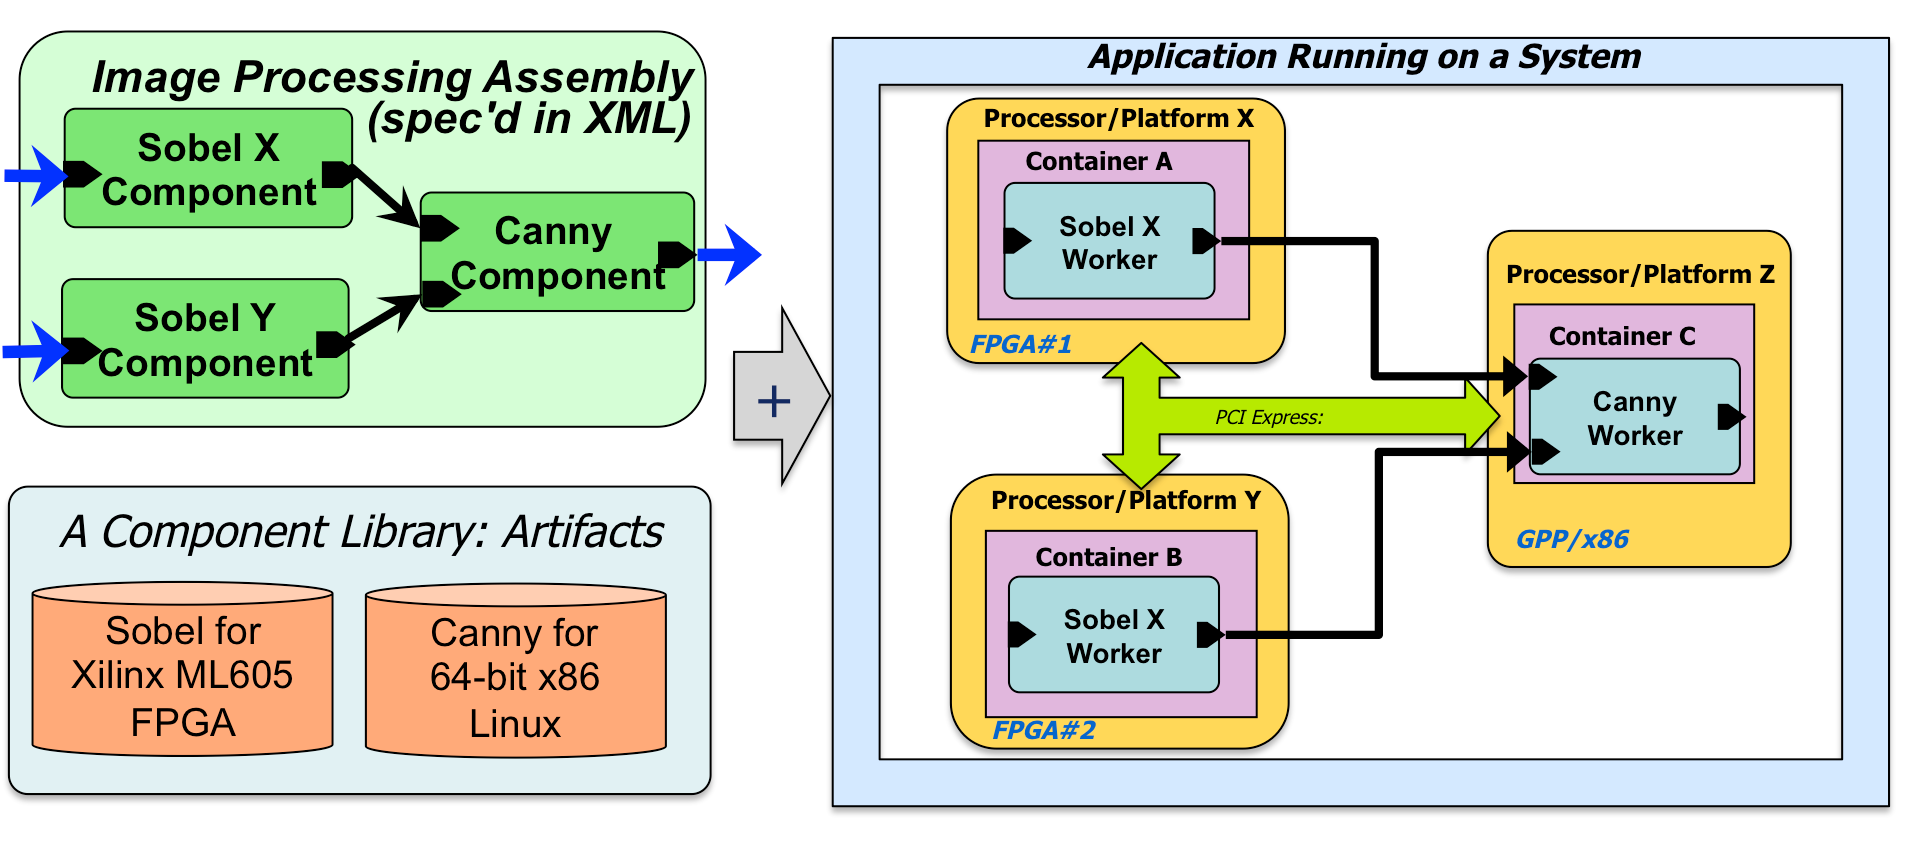
\includegraphics[width=1.0\linewidth]{Components.png}
 	\caption{Application of Components Deployed on a System}\label{fig:Components}
\end{figure}
\newpage
\section{OpenCPI Application Specification OAS XML documents}
This section defines the XML document format for describing OpenCPI applications. Such XML documents may be held in files or in text strings within a program. They describe a collection of component instances, along with their interconnections and configuration properties. An \hyperlink{OAS}{OAS} may be directly executed using the ocpirun utility program described below. An OAS may also be constructed and/or manipulated pro grammatically and dynamically, and executed using an API described in API for executing XML-based applications in C++/Python:\hyperlink{ACI}{ACI}. An OAS may also be constructed and/or manipulated programatically and dynamically, and executed using an API described in the section: \hyperlink{sec:API for executing XML-based applications}{API for executing XML-based applications}.\\


The primary contents of the OAS are component instances. When the author of an OAS specifies a component instance, they are referring to a component specification. They are saying: I need a component implementation that meets this specification. Normally, the OAS says only that, and does not say which particular implementation of that component spec (i.e. which worker) should be used. This allows the OAS to be used in a variety of different configurations of hardware and different libraries of component implementations. A very simple example of an OAS is below, showing an application that reads data from a file, adds 1 to each data value, and writes the result.\begin{ocpixml}
<application>
	<instance component='file_read' connect=add1>
		<property name='filename' value='test.input'/>
	</instance>
	<instance component='add1' connect=file_write/>
	<instance component='file_write'>
		<property name='filename' value='test.outputwrong'/>
	</instance>
</application>
\end{ocpixml}

Each instance specifies the component, some properties and a connection.
\subsection{Quick XML Introduction}
XML documents are text files that contain information formatted according to XML (Extensible Markup Language) syntax and structured according to a particular application-specific schema.The textual XML information itself is formatted into elements, attributes, and  textual content.  The OAS XML schema does not use or allow textual content at this time.  XML elements have attributes and child elements (forming a hierarchy of elements).  XML elements take two forms. The simpler one is when an element has nochild (embedded) elements and no textual content.  It looks like this (for element of type xyz with attribute abc): \begin{ocpixml}
<xyz abc=`123`/>
\end{ocpixml}
Thus the element begins with the: $<$ character and the element type and is terminated with the:/\/$>$ characters. Attributes have values in single or double-quotes.  Any white space, indentation, or new lines can be inserted for readability between the element name and attributes or between attributes.Thus the above example could also be: \begin{ocpixml}
<xyz
abc="123" 
/>\end{ocpixml}
When the element has child elements (in this case a child element of type ccc with attribute cat), 
it looks like:\begin{ocpixml}
<xyz abc=''123">
<ccc cat="345"/>
</xyz>\end{ocpixml}

In this case, the \emph{start} of the xyz element (and its attributes), is surrounded by \begin{verbatim}<>\end{verbatim} and the \emph{end} of the xyz element is indicated by \begin{ocpixml}
</xyz>
\end{ocpixml} 
An XML schema defines which elements, attributes, and child elements the document may contain. Every XML document has a single top-level element that must be structured (attributes and sub-elements) according to the schema.  An $<$extension$>$ child element is always legal and always ignored.  It can be used when tools want private embedded elements that are unknown to OpenCPI. An element can be entered directly (as above) or by referring to a separate file that contains that element. So the example above might have a file, \begin{verbatim}<ccc1.xml>\end{verbatim} containing: \begin{ocpixml}
<ccc cat="345"/>
\end{ocpixml}

And then a top-level file called "xyz1.xml" containing: 
\begin{ocpixml}
<xyz abc="123">
<xi:include href="ccc1.xm"l/>
</xyz> \end{ocpixml}
However, the schema specifies which elements are allowed to be top-level elements in any file.  All element and attribute names used in OpenCPI are case insensitive. All attributes are defined with specific data types and formats. When an attribute is defined as the boolean type, the default value (used when the attribute is not specified) is "false" unless otherwise noted. All element and attribute names are case insensitive.
\subsection{Top Level Element in an OAS: (application)}The top-level element in every OAS document (file or string) is the application element.  Application elements contain child elements that are either instance or connection, and have attributes that are name, done, package, and maxprocessors, these are described below.
\subsubsection{Name attribute (optional)}The name attribute of an application is simply used in various error messages and other debug log messages.  It has no functional purpose, only documentation and labeling.
\subsubsection{Done attribute (optional)}The done attribute identifies the instance within the OAS that is used to determine when the application is done executing.  When the indicated instance is done, then the whole application is considered done.  If this attribute is not supplied, the application is considered done when all its instances are done. The value of this attribute must match the name attribute of one of the instance elements, described below. For some applications, and some components, there is no definition or functionality of being done. In this case whatever mechanism started the application must decide when to stop it and shut it down.
\subsubsection{Package attribute (optional)}The package attribute of an application is used as a default package prefix for all instances in the assembly. Any instances component attribute that does not have a package prefix is assumed to be in the package indicated by this attribute. When not specified, the default package prefix for all components mentioned in the assembly is local. The prefix of the \hyperlink{core}{core} OpenCPI component library is ocpi.core.  If you are using mostly components in that library, you might include package=ocpi.core as an attribute.  If you are using only components specified in your own library of components (which has a default prefix of local), you could ignore this attribute and use no prefixes at all. See the component attribute of the instance element below.
\subsubsection{MaxProcessors attribute (optional)}The MaxProcessors attribute indicates the maximum number of processors(containers) that should be used to run the application.  When instances are allocated to processors, an algorithm decides which processor runs each instance.  If this attribute is not set, the default behavior is to spread the instances across available processors, and use a round-robin assignment policy when there are more instances than processors. If this numeric parameter is set, it limits the number of processors used, if possible.  If more are necessary to host the necessary workers, more will indeed be used in any case.  An example of when this attribute is not effective is when the availability of implementations of each instance dictate that more processors are needed, such as when the only implementation available for an instance is for a particular processor, which must then be used.
\subsection{Instance Elements within the Application Element}The instance element is used as a child of the application element to specify a component instance in the application.  It may have property child elements, and may have component, name, connect,selection, from, to and external attributes. For example:\begin{ocpixml}
<instance component='file\_read' connect="add1">
	<property name='filename' value='test.input'</>
</instance>\end{ocpixml}
The order of instance elements is significant for the purpose of assigning names to each instance when the instance element does not specify a name.  When applications are started, the instances in the application are started using ordering rules that do not depend on the ordering of instance elements in the OAS.  The detailed ordering rules are outside the scope of this document, but in general instances with no input ports (typically sources of data) are started last to avoid startup overrun conditions.
\subsubsection{Component attribute (required)} The component attribute of an instance specifies the component being instantiated.The value is a string used to find implementations for this instance, by searching in the available artifact libraries. It is the name assigned by the component developer to the component specification used as the basis for implementations.  Component specifications are themselves XML documents/elements called OCS (OpenCPI Component Specification). They have names (used to match this attributes value), and describe the ports and properties that apply to all implementations of that component. This attribute is required, and answers the question: what function should this instance perform? The process by which OpenCPI searches for implementations based on this attribute is described above. \\

This attribute may have a package prefix (ending in a period) to indicate which package contains the component specification indicated. If there is no prefix, the package prefix is taken from the default for the whole assembly, which is specified using the package attribute of the top-level application element.  If there is no package attribute in the application, and the component prefix is not present, the prefix "local" is used. This attribute provides the PackageID of the component by combining any prefix from the application's package attribute with its value if the value contains no periods. Package IDs are meant to be global identifiers constructed similar to Java package names.
\subsubsection{Name attribute (optional)}The name attribute of an instance is optional, and provides a unique identifier for the instance within the application. If it is not supplied, one is assigned to the instance. If there is only one instance in the application for a type of component (i.e. the component is used only once), the assigned instance name is the same as the component name (without package prefix). If more than one such instance (of the same component) exists in the application, the assigned name is the component name (without package prefix) followed by the decimal ordinal of that instance among all those for the same component. Such ordinals are assigned starting with 0. 
For example, in the example application above, there is one instance of the file\_read component, and thus its instance name would be file\_read.  If the application used file\_read twice (e.g. two different components were taking data from different files), the two instances would be named file\_read0 and file\_read1 in the order they occurred in the OAS.
\subsubsection {Connect attribute (optional)} Connecting instances together in an assembly can be done one of two ways.  Using the connect attribute of an instance is the simplest, but cannot express all connections.The connection child element of the application element can be used to express all types of connections which are described later.\\

The connect attribute defines exactly one connection from an output port of this instance to an input port of another instance. Its value is the name of the other instance. If this instance only has one output port and the other instance only has only one input port, then these are implied. The optional from attribute specifies the name of the output port of this instance if needed (if there are more than one), and the optional to attribute specifies the name of the input port of the other instance (if there are more than one). An example using all three attributes is:\begin{ocpixml}
<application>
    <instance component="psd"
    		connect=demod from=myout to="demod_in"/>
   <instance component="demod" selection=model=="rcc"/>
  </application>\end{ocpixml}
This simple connection method is useful for the many components that have only one output port.
\subsubsection{Selection attribute (optional)}\hypertarget{sec:Selection attribute (optional)} This attribute optionally specifies how to choose among alternative implementations when more than one is available. This capability also provides a way for the application to specify minimum conditions on the candidate implementations found in the library. The attribute value is an expression in the syntax of the C language, with all the normal operators, including the ?: ternary operator.  Logical expressions (e.g. \emph{"a == 1"}) return on true and 0 when false. The variables that may appear in the expression are either:
\begin{itemize}
\item Property names that have fixed (not runtime variable) values
\item Built-in identifiers that indicate well-known attributes of the implementation. \end{itemize}
The built-in identifiers are:
\begin{itemize}
	\item []{Model}:  the name of the \hyperlink{authoring model}{authoring model} of the implementation, e.g. rcc
	\item []{Platform}:  the name of the platform the implementation is built for, e.g. centos7 or ml605
	\item []{OS}: the name of the operating system the implementation is built for, e.g. linux
\end{itemize}
The value of the selection expression is considered an unsigned number, where a higher number is better than a lower number, and zero is considered unacceptable. For example, if the expression when evaluated for an implementation has a zero value, that implementation is not considered a candidate. A simple example might be: \begin{verbatim} model==''rcc''.\end{verbatim} This indicates that the model must be \emph{rcc} since otherwise the expressions value will be zero. \\
The example:\begin{ocpixml}
error_rate < 5 ? 2 : 1\end{ocpixml} 
indicates that the \emph{error\_rate} property is relevant and if less than 5, it is better than when greater than or equal to 5, but the latter is still acceptable. If there is no selection expression, the "score" of the implementation is 1, unless it has hard-wired connections to other collocated workers (e.g. on an FPGA). In this case, its value is 2.\\

An example of using the selection attribute is:\begin{ocpixml}
<application>
  <instance component="psd" selection=latency < 5/>
  <instance component="demod" selection=model=="rcc"/>
</application>\end{ocpixml}
It indicates that the \emph{psd} instance needs an implementation with latency less than 5, and the \emph{demod} instance must have an implementation with an authoring model of rcc.
\subsubsection{From attribute (optional)}This attribute is used to specify the name of the output port of this component instance in conjunction with using the connect attribute described above.
\subsubsection{To attribute (optional)} This attribute is used to specify the name of the input port of the other component instance in conjunction with using the connect attribute described above.
\subsubsection{External attribute (optional)} This string attribute is used to specify a port of the instance that is to be considered an external port of the entire application.  Its value is the name of this instances port that should be externalized.  The external application-level name of the port is the same as its own name on this instance.  To specify a different name, use the connection element described below. The name of this attribute is singular and distinct from the externals attribute described next.
\subsubsection{Externals attribute (optional)} This boolean attribute is used to specify that all unconnected ports of the instance are to be considered external ports of the entire application.  The external application-level names of the ports are the same as their own name on this instance. To specify different names, use the connection element described below.  Note that the name of this attribute is plural and distinct from the external attribute described previously.
\subsubsection{Worker attribute (optional)} This string attribute is used to specify a particular worker to use for this instance. Usage of this attribute is rare and generally not recommended in the OAS since it bypasses the automatic selection algorithm for choosing the worker based on available implementations and available containers.  The string value is the name of the worker without any suffix for authoring model or package name prefix.
\subsubsection{Property elements within the instance element (optional)} The property element is used as a child of the instance element to specify configuration property values that should be configured in the worker when the application is run, prior to the application being started. Within an instance element, some examples of property (child) elements are:
\begin{ocpixml}
	<instance component="psd">
  		<property name=size value="17"/>
  		<property name=symmetric value="true"/>
	</instance>\end{ocpixml}
Properties can only be set if they are specified in the spec with access as \emph{initia} or \emph{writable}.  Property values may also be set outside the OAS (on the command line or as a runtime-parameter).  Using these mechanisms outside the OAS makes the OAS more reusable since it can be used with different property values settings.
\subsubsection{Name attribute (required)}The name attribute of a property element must match the name of a property of the specified component. I.e., it must be one of the defined configuration properties of the component. Component specifications define properties that are common to all implementations of a component. Component implementations (workers) can also define additional properties that are specific to that implementation, but mentioning such properties will only be accepted if the selected implementation has them. Otherwise an error results.
\subsubsection{Value attribute (one of value or valueFile (required)} The value attribute is the value to be assigned to the configuration property of the worker just before being started.  The attributes value must beconsistent with the data type of the property in the component specification.  I.e. if the type of the property is, ulong, then the attributes value must be numeric and not negative. The complete syntax of property values is described in the \hyperlink{sec:Property Value Syntax and Ranges}{Property Value Syntax and Ranges} section.
\subsubsection{ValueFile attribute (one of  value or valuefile is required)} The ValueFile attribute is the name of a file containing the value to assign to the property.  Using this attribute, rather then the value attribute, is convenient when the value is large, such as when the propertys value is an arrays of values.  When valueFile is used, all new lines in the file are interpreted as commas. The complete syntax of property values is described in \hyperlink{sec:Property Value Syntax and Ranges}{Property Value Syntax and Ranges} section.
\subsubsection{DumpFile attribute (optional)} The DumpFile attribute is the name of a file into which the value of the property will be written after execution (when using the ocpirun utility program described below). When DumpFile is used, all commas in the value are replaced by new lines in the written file. The complete syntax of property values is described in \hyperlink{sec:Property Value Syntax and Ranges}{Property Value Syntax and Ranges} section.
\subsubsection{Delay attribute (optional)}  Normally property settings are made before the application starts, but it is possible for a property value to be set after the application starts.  This delay attribute specifies when the property value should be set after the application starts.  A value of zero means as soon as possible after the application starts.  Any value greater than zero indicates the amount of time to wait (in seconds) after the application starts, before setting the value.\\

The delay values are in units of seconds and may be floating point.  Thus 5e-6 would indicate 5 microseconds.

Multiple delays and values may be specified for a property to indicate a timed sequence of property settings.  This is done by inserting multiple set elements as child elements of the property element.  Each set element may have its own delay and indicate the value to be set using the value or valuefile attributes. Here is an example that sets a property's value 5 seconds after the application starts, and then sets a different value 10 seconds after the application starts.\begin{ocpixml}
 <application>
      <instance component='mycomp'>
      		<property name='control'>
      			<set value='123' delay='5'/>
      			<set value='345' delay='10'/>
      		</property>
      		<property name='other' delay='20' value='789'/>
      </instance>
</application>\end{ocpixml}
\subsection{Property Elements within the Application Element (optional)} Property elements at the top level of an application (rather than under an instance element), represent properties of the application as a whole.  They are essentially a mapping from a top-level property name to a property of some instance in the assembly.This provides a convenient way to expose properties to the user of an application without requiring them to know the internal structure of the application.  For example:\begin{ocpixml}
      <application>
        	<property name='infile' instance='file_read' property='filename'/>
        	<instance component='file_read' connect=add1>
        		<property name='filename' value='test.input'/>
        	</instance>
        	<instance component='add1' connect=file_write/>
        	<instance component='file_write'>
        		<property name='filename' value='test.outputwrong'/>
        	</instance>
      </application>\end{ocpixml}
The above example provides an application-level property named, infile, which is mapped to the filename property of the file\_read component instance.  In addition to the attributes listed here, the top-level property elements also accept the value, valueFile, and dumpFile attributes described in the previous section.
\subsubsection{Name attribute (required)} The name attribute of an application-level property is the name that users of the application will use to read, write or display the value.  If the property attribute just below is not present, then this name is also the name of the instances property.
\subsubsection{Instance attribute (required)}This attribute specifies the name of the instance that actually implements this property for the application.  It is the instance that the application-level property is mapped to.
\subsubsection{Property attribute (optional)} If the application-level name of this property is not the same as the instances property to which is it mapped, this attribute is used to specify the actual property of the instance. It is a string property that must match a property of the instance.
\subsection{Connection Elements within the Application Element (optional)} Connecting instances together in an assembly can be done one of two ways. Using the connect attribute of an instance is the simplest (described above), but cannot express all connections. The connection child element of the application element can be used to express all types of connections.  It describes connections among ports and also with "the outside world", i.e. external to the application.  The connection element has optional name and transport attributes, and port and external child elements. An example of an application with some connections is:\begin{ocpixml}
    <application done='file_write'>
      <instance component='file_read'/>
      <instance component='bias'/>
      <instance component='file_write'/>
      <connection transport=socket>
           <port instance='file_read' name='out'/>
           <port instance='bias' name='in'/>
      </connection>
      <connection>
           <port instance='bias' name='out'/>
           <port instance='file_write' name='in'/>
      </connection>
    </application>\end{ocpixml}

The first connection connects the out port of the file\_read instance to the in port of the bias instance, and specifies that the connection should use the socket transport mechanism.  The second simply connects the out port of the bias instance to the in port of the file\_write instance. This second connection could have been more simply accomplished by using the connect attribute on the bias instance.
\subsubsection {Name attribute (optional)} This attribute specifies the name of the connection. It is only used for documentation and display purposes and has no specific other function.  If it is not present, a name is assigned according to the conn \begin{verbatim}<n> pattern, where <n> \end{verbatim}is the number of the connection in the application (0 origin).  If the connection is thought of as a "wire", this is the name of the wire that is attached to various other things (instance ports and external ports).
\subsubsection {Transport attribute (optional)}  This attribute specifies what transport mechanism should be used for this connection. OpenCPI supports a variety of transport technologies and middlewares that convey data/messages from one instances port to another. 

Normally, the transport mechanism is chosen automatically based on which ones are available and optimal. This attribute allows the application to override the default transport mechanism and force the usage of a particular one. 
The transport attributes supported at the time of this document update are:\\

\begin{table}[h!]
\caption{Transport Attribute Options}
\renewcommand*{\arraystretch}{2.5}
\center
\begin{tabular}{|c|p{14cm}| }
\hline \emph{Name} & \emph{Description}\\
\hline 
pio & Programmed I/O using shared memory buffers between processes\\
\hline
pci & DMA or PIO over the PCI Express bus/fabric \\ 
\hline   
ofed & RDMA using the OFED software stack, usually for InfinibandOpenCPI \\ 
\hline 
socket & RDMA using TCP/IP sockets \\ 
\hline 
ether & RDMA using Ethernet (link layer) frames \\ 
\hline 
udp & RDMA using UDP/IPRDMA using Ethernet (link layer) frames \\ 
\hline
\end{tabular}
\end{table}
Some of these transport mechanisms are only available if specifically installed in a system.
\emph{See the OpenCPI Installation Guide.}
\subsubsection{Port elements within the connection element (optional)} This element is used to specify a port that this connection should be attached to. The most common use of this element is to specify the consumer and producer of the connection, using a {port} element for each, within the same connection element. However, port elements can be used to indicate more than two ports on the same connection, when there are multiple consumers for the connection (currently not supported).
\subsubsection{Instance attribute (required)} This attribute specifies the name of the instance of the port to be attached to this connection. This instance name is used along with the name attribute to specify the port.
\subsubsection{Name attribute (required)} This attribute specifies the name of the port that should be attached to this connection. This port name is scoped to the instance defined in the instance attribute of the connection element.
\section{The ocpirun Utility Program for Executing XML-based Applications} \label{sec:The ocpirun utility program for executing XML-based applications} The simplest way to run an OpenCPI application is to describe it in an XML file (an OAS as described above), and run it using the command-line utility ocpirun. This command reads the OAS file and runs the application.  E.g., if the OAS was in a file named \begin{ocpixml}
myapp.xml \end{ocpixml}
the following command would run it: \begin{ocpixml}
ocpirun myapp\end{ocpixml}

With some typical options, the command would be: \begin{ocpixml}
ocpirun -v -d -t 10 myapp\end{ocpixml} 

This would be verbose during execution, dump property values after initialization and after execution, and limit execution to 10 seconds. The execution ends when the application described in the OAS is done or the provided time duration is exceeded.  As mentioned above, an application is done either when all its workers indicate they are done or when a single worker, identified using the done attribute in the OAS, says it is done.  The ocpirun utility also has an option to stop execution after a fixed period of time.\\

There are a number of options to ocpirun, which are all printed in the help message when it is executed with no arguments.  Options that are "Bool", have no value:  their presence indicates true.  When an option has a value, the value can immediately follow the option letter, or be in the next argument.  There are general options, function options and options that refer to a specific instance in the application.  These are all described below.  \\
Some options can also be expressed as XML attributes in the OAS and some may also be used in the Application Control Interface described below in ACI. A complete alphabetical option summary, for all three ways of indicating options, is in \hyperlink{sec:Execution Options Summary - Alphabetical}{Execution Options Summary - Alphabetical}. When ocpirun executes the application, it must make deployment decisions, which decide, for each instance:
\begin{itemize}
\item which worker in which compiled artifact should be used
\item which container should it run in
\end{itemize}
\section{General Options for ocpirun}\label{sec:General Options to ocpirun}
There is an automatic built-in algorithm to make these decisions, as well as a number of options described below that override or guide the automatic deployment algorithm.
\renewcommand*{\arraystretch}{2.5}
\begin{center}
\begin{longtable}{|l|c|c|p{11cm}|}
\caption{General Options to ocpirun} \label{tab:long} \\
\hline \multicolumn{1}{|c|}{Name} & \multicolumn{1}{c|}{Letter} & \multicolumn{1}{c|}{Data Type}& \multicolumn{1}{l|}{Description} \\ \hline 
\endfirsthead
\multicolumn{4}{c}%
{{\bfseries \tablename\ \thetable{} -- continued from previous page}} \\
\hline 
\hline \multicolumn{1}{|c|}{Name} & \multicolumn{1}{c|}{Letter} & \multicolumn{1}{c|}{Data Type}& \multicolumn{1}{l|}{Description} \\ 
\hline  
\endhead
\hline \multicolumn{4}{|c|}{{Continued on next page}} \\ \hline
\endfoot
\hline \hline
\endlastfoot
 dump & d & Bool & Dump all readable properties after initialization, 
and again after execution, to stderr\\ 
\hline
 verbose & v & Bool & Be verbose in describing what is happening\\ 
\hline
hex & x & Bool & Print numeric property values in hex, not decimal\\ 
\hline
uncached & U & Bool & When dumping property values do not use cached values that are remembered by ocpirun when they are written.Actually query the worker in its execution environment (which is much more expensive)\\ 
\hline
processors & n & ULong & Create this many RCC containers (default is 1) \\ 
\hline
log-level & l & ULong & Set the OpenCPI log level to the given level. Overrides any value of the OCPI\_LOG\_LEVEL environment variable.\\
\hline
duration & t & ULong & Stop execution after this many seconds. If the application is not done before this amount of time, the application stops and is considered a successful execution (with the ocpirun exit code being zero).\\ 
\hline 
timeout & O & Ulong & If the execution in seconds exceeds this amount, the application is stopped and is considered a failure, with the ocpirun exit code being 1\\
\hline 
 server& S & String & A server (name or IP address) to explicitly contact for remote containers whether or not the remote option is not specified.  
This option may be specified multiple times\\ 
\hline 
remote & R & Bool & Automatically discover servers offering remote containers using multicast UDP\\ 
\hline
 deployment & {} & String & Specify a filename to read for deployment decisions, rather than using the built-in deployment algorithm.  See deploy-out\\ 
\hline 
deploy-out & {} & none & The name of a file in which to record deployment decisions for this execution, in XML format. Such an output file can be supplied later in the deployment option, to use the exact deployment recorded from a previous run (or from a no execute function as defined below)\\ 
\hline
library-path& none & String&Override the OCPI\_LIBRARY\_PATH environment variable.\\ 
\hline 
dump-file & none & String &The name of a file in which to record the final property values in machine-parseable form.\\ 
\hline 
component & none & Bool & Indicates that the first non-option argument is in fact a component name for a single-\hyperlink{component application}{component application} rather than the file name of an OAS.\\ 
\hline 
no-execute & none & Bool & Indicates that the application should not really execute, but all deployment decisions should be made, and if requested, recorded in the file indicated by the deploy-out option.\\ 
\hline
dump-platform & M & Bool& Dump all platform worker and device worker properties, in addition to properties of the workers in the application.\\
\hline
\end{longtable}
\end{center}
\subsection{Function Options for ocpirun} The function options tell the ocpirun command to perform certain functions other than executing the application. Options only relating to these non-execution functions are also listed here in the following table.
\renewcommand*{\arraystretch}{2.5}
\begin{center}
\begin{longtable}{|l|c|c|p{11cm}|}
\caption{Function Options to ocpirun} \label{tab:long} \\
\hline \multicolumn{1}{|c|}{Name} & \multicolumn{1}{l|}{Letter} & \multicolumn{1}{l|}{DataType}& \multicolumn{1}{l|}{Description} \\ \hline 
\endfirsthead
\multicolumn{4}{c}%
{{\bfseries \tablename\ \thetable{} -- continued from previous page}} \\
\hline \multicolumn{1}{|c|}{Name} & \multicolumn{1}{l|}{Letter} & \multicolumn{1}{l|}{Data Type}& \multicolumn{1}{l|}{Description} \\ 
\hline  
\endhead
\hline \multicolumn{4}{|c|}{{Continued on next page}} \\ \hline
\endfoot
\hline \hline
\endlastfoot
list & c & Bool & List all available containers, including those discovered 
on the network (if the -R or -S options are specified).  Assign each a number for easy assignment with the -c instance option described below.  The application is still executed if an application filename argument is specified after the options.\\ 
\hline
only-platforms & none & Bool & Modifies the list command to only print available platforms, listing any available platform only once even if there is more than one container with the same platform type.\\ 
\hline
list-artifacts & A & Bool & This function searches for all artifacts for any of the listed targets or platforms \begin{verbatim}(using the –target, or -r option),\end{verbatim} based on OCPI\_LIBRARY\_PATH, and prints the list to stdout.  Used to collect artifacts for a specific system.\\  
\hline
list-specs & none & Bool & This function searches for all artifacts for any of the listed targets or platforms\begin{verbatim} (using the –target, or -r option),\end{verbatim} based on OCPI\_LIBRARY\_PATH, and prints the list to stdout.  Used to collect available specs for a specific system.\\  
\hline
target & r & String & A target  \begin{verbatim}<os>-<os-version><arch>\end{verbatim}, or platform for the list-artifacts and list-specs commands.  May be specified more than once.\\  
\hline
no-execute & none & Bool & After the normal process of deciding, for each instance, what container it will run on, and what artifact will be used to run it, stop short of actually allocating any resources or performing execution.  This option can be used as a \emph{dry run} to see what would happen, and with the deploy-out option, record the deployment decisions in an XML file. \\ 
\hline
\end{longtable}
\end{center}
\subsection{Instance Options for ocpirun}\label{subsec:Instance Options for ocpirun}The instance options allow a value to be specified that applies to either all instances or just one instance. \\All these options take string values and the values are of the form:\begin{ocpixml}
<instance-name>=<value>\end{ocpixml}
So the option:\begin{ocpixml}
<-m=rcc> \end{ocpixml}
would set the m option (the authoring model) for all instances to rcc. 
While the option:\begin{ocpixml}
<-mctl=rcc> \end{ocpixml}
would set the m option for the ctl instance to be rcc. \\

These options can appear more than once to indicate options for different instances. If you specify an instance with an empty value e.g.\begin{ocpixml}
<-mctl=> \end{ocpixml} it unsets any previous default , such as, \begin{ocpixml}
<-m=rcc> \end{ocpixml}

So the following example would say that all instances have the rcc model except filter:\begin{ocpixml}
<-m=rcc-mfilter> \end{ocpixml}

These options typically provide constraints on the deployment algorithm to only consider certain workers or certain containers. The following table,{Instance Options to ocpirun), lists all instance options.
\begin{table}[h]
\caption{Instance Options for ocpirun}\label{tab:Instance Options to ocpirun}
\renewcommand*{\arraystretch}{2.5}
\center
\begin{tabular}[c]{|l|c | p{12cm}|}
\hline
\emph{Name} & \emph{Letter} & \emph{Description}\\
\hline
container & c & Assign the instance to a specific container, using the name or number from the listing of the -c command.
Examples:  \begin{ocpixml}
<-cfft=1 -cfir=rcc2>\end{ocpixml}\\ 
\hline  
model	& m	& Specify the authoring model of the named instance.  This creates a constraint that the worker used for this instance must have this model. Examples:  \begin{ocpixml}
<-m=hdl -m fft=rcc>\end{ocpixml}\\ 
\hline 
platform & P	& Assign instance only to containers for this platform type (see output from -C)
Examples:  \begin{ocpixml}
<-Pfft=ml605 -P=centos7>\end{ocpixml}\\   
\hline 
property	& p	& Set the value of a property.The value of the option is either:
\begin{ocpixml}
<property-name>=<value>\end{ocpixml}for application-level properties, or 
\begin{ocpixml}
<instance-name>=<property-name>=<value>\end{ocpixml} 
property value settings. See below for more details. \\ 
\hline 
selection & s & Set the selection expression for the instance.  See below for more details.  
Example, to request that for the ctl instance, only workers with the snr property less than 5 are used: -s 'ctl=snr $<$5' See the \hyperlink{sec:Selection attribute (optional)}{Instance Selection attribute section}.\\ 
\hline 
worker & w & Specify the name of the worker (specific implementation) to be used for the instance.
Note this does not include model suffix or package prefix.\\ 
\hline
\end{tabular}
\end{table}

\subsubsection{Setting Properties in the Application}The property setting option (-p) can set an application-level property rather than an instance property.  Application-level properties are those specified using the property element at the top level of the OAS, as a child element of the application element. Application-level properties have an application-level name that is mapped in the OAS to the underlying instance and property name. When setting a top level application property value, the form of the option is: \emph{-p control = 5 }which sets the application level control property to the value 5. When specifying the property value of an instance, the form of the option is: -p file\_read=filename=myinput.data which sets the filename property value of the file\_read instance to: myinput.data. Property values must be consistent with the data types defined in the component specification.  The syntax for all data types is described in the \hyperlink{sec:Property Value Syntax and Ranges} {Property Value Syntax and Ranges} section below.
\newpage
\subsubsection{Instance options that apply to the ports of instances} There are several options that apply to specific ports of instances in the application.These options modify default behavior for the communications occurring at that port.When a port is connected to a port of another instance, the connection is between two ports.Some of the port options apply to only one end (one port) of the connection,while others apply to the connection as a whole and thus apply to both the mentioned port as well as the port it is connected to. The syntax of port options is: \begin{ocpixml}
<instance-name>=<port-name>=<value> \end{ocpixml}
If the option is port-specific (for only one end of the connection), the value is applied to that port.  If the option is for connections, the value is applied to the indicated port as well as the port it is connected to. The following table, Instance port options to ocpirun, lists all instance port options.
\begin{table}[h!]
\caption{Instance port options to ocpirun}
\renewcommand*{\arraystretch}{2.5}
\begin{tabular}[c] {| l | c | p{12cm}|}
\hline
\emph{Name} & \emph{Letter} & \emph{Description}\\
\hline
 buffer-count & B & Specify the number of buffers at this instance port (not for all ports of the connection).  The default is usually 2.  This option allows the number of buffers to be different each end of the connection. \\ 
\hline  
buffer-size & Z	& Specify the the buffer size for the connection (for this port and the port it is connected to).  The default is usually determined by a combination of the protocol used on the connection and other system constraints.\\ 
\hline  
transport & T	& Specify the transport technology used for the connection (for this port and the port it is connected to).  This applies when using remote containers.\\ 
\hline
\end{tabular}
\end{table}
\subsection{External Port Options to ocpirun}\label{subsec:External port options to ocpirun}
Several options apply to the external ports of the application (which are not connected to anything else in the OAS). They use the syntax: \begin{ocpixml}
<externalport>=<value>\end{ocpixml}
\begin{table}[h!]
\caption{External Port Options to ocpirun}\label{External Port Options to ocpirun}
\renewcommand*{\arraystretch}{2.5}
\begin{tabular}[c]{| l | c | p{12cm}|}
\hline \emph{Name} &\emph{Letter} & \emph{Description}\\
\hline
file & f & Specify the name of the file to connect to this external port.  This inserts a file\_read or file\_write component into the application, and connects it to the named external port. These utility components are described in \emph{Utility Components for Applications}.  This allows an OAS with external ports to be used with those ports connected to files while also allowing it to be used with those same ports connected to an ACI application (described in \hyperlink{API for executing XML-based applications in C++/Python:  ACI} {API for executing XML-based applications in C++/Python:  ACI} \\ 
\hline  
buffer-count & B & Specify the buffer count for this external port\\ 
\hline   
buffer-size	& Z	& Specify the the buffer size for this external port (for this port and the port inside the OAS it is connected to).  The default is usually determined by a combination of the protocol used on the connection and other system constraints.\\ 
\hline  
transport &T& Specify the transport technology used for the connection (for this port and the port it is connected to).  This applies when using remote containers.\\ 
\hline
\end{tabular}
\end{table}
\newpage
When the file option is used to connect an external port to a file, the detailed property settings for the inserted file\_read or file\_write components may be supplied after the filename using the URL option syntax of:\begin{ocpixml}
<name>=<value>;<name2>=<value> \end{ocpixml}
So, if an external port whose name was input was to be connected to the file myinput.txt with the opcode option set to 2 and the suppressEOF option set to false, the option syntax would be:\begin{ocpixml}
<-f 'input=myinput.txt?opcode=2;suppressEOF=false' >\end{ocpixml}
Note that the option value is quoted since the question mark and semicolon are shell metacharacters.
\subsection{Simulation Options for ocpirun} The simulation options are used to control containers that are running HDL/FPGA simulators.  Any available simulators are used as normal containers during the deployment algorithm which decides what artifacts are used and where instances will run. Available simulators are included in the output of the --list (or -C)  function of ocpirun. \\
These options are normally used during HDL/FPGA component development and testing, but are listed here in Simulation Options to ocpirun for completeness. They are described in more detail in the \emph{OpenCPI HDL Development }document.
\begin{table}[h!]
\caption{Simulation Options for ocpirun}\label{Table Simulation Options to ocpirun}
\renewcommand*{\arraystretch}{2.5}
\begin{tabular}[c]{| l | c | p{12cm}|}
\hline\emph{ Name} & \emph{Letter} & \emph{Description}\\ 
\hline    
sim\_dir & none & The name of a directory where simulation outputs will be placed.  The default is simulations, relative to where ocpirun itself is running.\\ 
\hline  
sim-ticks & none & The number of simulation clock cycles to execute or until the application is done.\\ 
\hline
\end{tabular}
\end{table}
\section {Property Value Syntax and Ranges}\hypertarget{sec:Property Value Syntax and Ranges}{Property Value Syntax and Ranges}
This section describes how property values are formatted to be appropriate for their data types.  Property values for applications occur in three places:
\begin{itemize}
\item the value attribute of property elements in the OAS XML
\item on the ocpirun command line when options are used to set property values
\item in C++ when the ACI is used to apply property values to applications the ACI is described in \hyperlink{sec:API for executing XML-based applications} {API for executing XML based Applications}
\end{itemize}The syntax accepted depends on the type of the property whose value is being set, and certain quoting requirements depend on the context where the value is specified.\\

In \emph{XML attributes}: Attribute values in XML syntax are in single or double quotes.  The property value syntax described below is used inside these quotes (in the OAS).  To have quotes inside XML attribute values, the other type of quotes is used to delimit the attribute value.  In either case, inside the quoted attribute value, the \& and $<$ characters must be escaped using the official XML notations:\& amp; for \& and \& lt; for $<$ If both types of quotes must be in an attribute value, then the official XML escape sequences for the quotes can be used:\& quot; for double quote, and \& apos; for single quote.\\

\emph{On the shell command line}: Similarly, when used on the command line for ocpirun, the shell quoting rules are different than in XML.  If the property value has no single quotes at all, then using single quotes for the shell command line argument is the most convenient when any of the shell's metacharacters are in the property value. The shell metacharacters are these: | \&  ;  (  )  $<$$>$ *  ?  [  ]  {  }  space  tab. If single quotes are in the value, or if shell variable or history expansion is required, the QUOTING section of the shell\/bash manual page defines how to escape them.\\

\emph{In a C++ program}:  In C++, the values will be defined in double-quoted string literals, where only double-quote characters and backslash characters must be escaped by preceding them with a backslash. These XML/shell/C++ rules are applied after the value is constructed according to the general property value syntax defined below. Property values are also used when creating component specifications and workers. That usage is described in the \emph{OpenCPI Component Development Guide} but the format is as described here.
\subsection {Values of \emph{Unsigned} Integer Types:  \emph{uchar, ushort, ulong, ulonglong}} These numeric values can be entered in decimal, octal with leading zero, or hexadecimal with leading 0x.  The limits are the typical ranges for unsigned 8, 16, 32, or 64 bits respectively. The uchar type can also be entered as a value in single quotes, which indicates that the value is an ASCII character, with backslash escaping as defined in the C language. The syntax inside the single quotes is as described for the char type below.
\subsection{Values of \emph{Signed} Integer Types: \emph{short, long, longlong}} These numeric values can be entered in decimal, octal with a leading zero, or hexadecimal with a leading 0x, with an optional leading minus sign to indicate negative values.  The limits are the typical ranges for signed 16, 32, or 64 bits respectively.
\subsection{Values of the Type:\emph{char}}This type is meant to represent a character, i.e. a unit of a string.  In software, it is represented as a signed char type, with the typical numeric range for a signed 8-bit value. The format of a value of this type is simply the character itself, with the typical set of escapes for non-printing characters, as specified in the C programming language and IDL:\begin{verbatim}
\n  \t  \v  \b  \r  \f  \a  \\  \?  \’  \”  \end{verbatim}
A series of 1-3 octal digits can follow the backslash and a series of 1-2 hex digits can follow \begin{verbatim}\x\end{verbatim} OpenCPI adds two additional escape sequences as a convenience for entering signed and unsigned decimal values of type char. The sequence:\begin{verbatim}\d \end{verbatim}may be followed by an optional minus sign (-) and one to three decimal digits, limited to the range of -128 to 127.  The sequence \begin{verbatim}\u \end{verbatim} can be followed by one to three decimal digits, limited to the range of 0 to 255. These escapes can also be used in a string value. Due to the requirements of the arrays and sequence values (see below), the backslash can also escape commas and braces, i.e.: \begin{verbatim}  \,    \{    \} \end{verbatim}  
\subsection{Values of the Types:  \emph{float and double}}These values represent the IEEE floating point types with their defined ranges and precision.  The values are those acceptable to the ISO C99 {strtof and strtod} functions respectively.
\subsection{Values of the Type:  \emph{bool}} These values represent the Boolean type, which is logical true or false.  The values can be case insensitive: true or 1 for a true value, and false or 0 for a false value.
\subsection{Values of the Type: \emph{string}} These values are simply character strings, but also can include all the escape sequences defined for the char type above.  Due to the requirements of arrays and sequence values, the backslash can also escape commas and braces \begin{verbatim} (\, and \{ and \} )\end{verbatim} Double quotes may be used to surround strings, which protects commas, braces and leading white space. To be interpreted this way, the first character must be a double quote. Two double quotes can represent an empty string.
\subsection{Values in a \emph{Sequence} Type} Values in a sequence type are comma-separated values.  When the type of a sequence is char or string, backslash escapes are used when the data values include commas.
\subsection{Values in an \emph{Array} Type} When a value is a one-dimensional array, the format is the same as the sequence, with the number of values limited by the size of the array.  If the number of comma-separated values is less than the size of the array, the remaining values are filled with the null value appropriate for the type.  Null values are zero for all numeric types and the type char.  Null values for string types are empty strings.
\subsection{Values in \emph{Multidimensional} Type}For multidimensional arrays or sequences of arrays, the curly brace characters (\{ and \}) are used to define a sub-value.  For example, a sequence of 3 elements, each consisting of arrays of length 3 of type char, would be:\begin{ocpixml}
<{a,b,c},{x,y,z},{p,q,r}>\end{ocpixml}
This would also work for a 3 x 3 array of type char.  Braces are used when an item is itself an array or sequence, recursively.
\subsection{Values in \emph{Struct} Type}Struct values are a comma-separated sequence of members, where each member is a member name followed by white space, followed by the member value.  A struct value can be sparse, i.e. only have values for some members. If the struct type was: \begin{ocpixml}
<struct long el[2][3]; string m2; char c; };  // C pseudo code>\end{ocpixml} 
A valid value would be:\begin{ocpixml}
<{1,3,2},{4,5,6}}, c x >\end{ocpixml}
This struct value would not have a value for the m2 member. Unmentioned members have null values.
\subsection{Expressions in \emph{Property} Values}Both numeric and string typed scalar values can be specified using an expression syntax and operator precedence from the C language, where any parameter property with a value can be accessed as a variable.  All C expression operators can be used except the comma operator, assignments or self-increments/decrements.  The conditional operator using ? and : is supported. Expressions can be used as elements of arrays or sequences, or as structure member values. For example, if the nbranches property was a parameter, a valid expression might be: \begin{ocpixml}
<nbranches == 0x123 ? 2k-1 :0177>\end{ocpixml}
\subsubsection{Numeric Values}The numeric constant syntax is typical C language syntax (integer and floating point), with the following additions:\begin{itemize}
\item Integers with explicit radix after a leading 0 can use 0t for base 10 and 0b for base 2, in addition to the normally used 0x for base 16 and no letter for base 8. All these prefixes can be applied to the fraction and exponent for floating-point syntax.
\item Integers can use a letter suffix of K, M, or G, upper or lower case, indicating \begin{ocpixml}
<2^10,  2^20 or 2^30>\end{ocpixml} respectively.  
E.g. \begin{ocpixml}
2k-1 is 2047\end{ocpixml}
\item All arithmetic is done using a numeric data type exceeding the range and precision of uint64\_t, int64\_t and double, and then assigned to the actual data type of the property.
\item The ** binary operator (pow) from the python and FORTRAN languages is also supported.\end{itemize}When the value of the expression is assigned to the property value, it is range checked for validity.  Boolean properties are set to true if the value is non-zero.  Fractions are discarded when assigning values to integer types.\\
\subsubsection{String Values}Within expressions, string constants (using double quotes as in C) can be used in expressions using string-typed parameters. All comparison operators are case sensitive and result in boolean numeric values (0 or 1).  All operators requiring boolean values \begin{ocpixml} 
<!, ||, &&, ?:> \end{ocpixml} use the length of the string (zero being false, otherwise true).  The + operator concatenates strings. There is no implicit or explicit conversion between string values and numeric values. So if sparam is a string-typed parameter with the value abc, then this expression has the numeric value of 1: \begin{ocpixml} 
<sparam =="abc">\end{ocpixml}. This expression would have the string value \begin{ocpixml}
<xyz_abc: "xyz_" + sparam>\end{ocpixml}
\subsubsection{Expressions used for String Values}To distinguish when a string value is an expression, as opposed to a string that might look like an expression, the string value must have a special prefix of \begin{verbatim}\: \end{verbatim}So if a property (or sequence/array element or structure member) is a string type, any value assigned to it is considered not to be an expression by default.  To make the string value interpreted as an expression, use the \begin{verbatim}\: prefix. \end{verbatim} So if sparam is a parameter with value \begin{ocpixml}
<abc>\end{ocpixml}
then specifying the property's string value:\begin{ocpixml}
<sparam+xyz>\end{ocpixml} 
would simply define that exact string (with plus sign and double quotes included) but if the string value was \begin{ocpixml}
<sparam+xyz>\end{ocpixml}
then it would be interpreted as an expression, and the actual string value would be:\begin{ocpixml}
<abcxyz>\end{ocpixml}
\section{Utility Components for Applications}\label{sec: utility components for applications}  There are several built-in components that are always available that application developers use frequently.  These are listed in this section, along with the available implementations.  Their availability on a given platform depends on whether they have been built for that platform and whether artifacts are available in the path specified by the OCPI\_LIBRARY\_PATH environment variable. All of these utility components are in the ocpi.core package, so using them usually involved specifying the instance's component attribute to \begin{verbatim}ocpi.core. <component>\end{verbatim} 
If most of the components in the application are in this package it may be more convenient to simply set the package attribute for the whole application.
\subsection{File\_Read Component that Reads Data or Messages from a File} The File\_Read component injects file-based data into an application.  It is normally used by specifying an instance of the File\_Read component, and connecting its output port to an input port of the component which will process the data first.  The name of the file to be read is specified in a property. \\

This component has one output port whose name is out, which carries the messages conveying data read from the file.  There is no protocol associated with the port, so that it is agnostic as to the protocol of the file data and the connected input port. This component has two modes of operation:  data streaming and messaging.
\subsubsection{Data Streaming Mode} In data streaming mode, the contents of the file becomes the payloads of a stream of messages, each carrying a fixed number of bytes of file data (until the last) and all with the same opcode.  The length and opcode of all output messages are specified as properties.\\

If the number of bytes in the file is not an even multiple of the message size the remaining bytes are sent in a final shorter message.  The granularity of messages can also be specified.  This forces the message size to be a multiple of this value and forces truncation of the final message to be a multiple of this value.  The default granularity is 1.
\subsubsection{Messaging Mode} In messaging mode, the contents of the file are interpreted as a sequence of defined messages, with an 8-byte header in the file itself preceding the data for each message. This header contains the length and opcode of the message, with the data contents of the message following the header.  The length can be zero, meaning that a message will be sent with the indicated opcode, and the length of the message will be zero.
The first 32-bit word of the header is interpreted as the message length in bytes, little-endian.  The next 8-bit byte is the opcode of the message, followed by 3 padding bytes. 
E.g. in the C language (on a little-endian processor):\begin{ocpixml}
<struct {
 uint32\_t messageLength;
 uint8\_t  opcode;
 uint8\_t  padding[3];
    };>\end{ocpixml}
This format of messages in a file is the format produced by the File\_Read component when in messaging mode, described next. If the end of the file is encountered while reading a message header, or while reading the header-specified length of the message payload, an error will be reported and the component will terminate.
\subsubsection{End of File Handling} When the File\_Read component reaches the end of its input file, it will do one of three things:\begin{itemize}
\item send a zero-length message with an opcode set by the opcode property (default)
\item declare itself to be done with no further action, when the \emph{suppressEOF} property is true
\item restart reading at the beginning of the file, when the \emph{repeat} property is \emph{true}
\end{itemize}
\subsubsection{Properties of the File\_Read Component}
\begin{table}[h!]
\caption{Properties of the File\_Read Component}
\renewcommand*{\arraystretch}{2.5}
\begin{tabular}[c]{|c|c|c|c|c|p{5cm}|}  
\hline \emph{Name} & \emph{Read Access} & \emph{Write Access} & \emph{Default} & \emph{Type} & \emph{Description}\\ 
\hline
fileName & Impl & Initial & none & String &	Name of file to be read\\ 
\hline  
messagesInFile & Readable & Initial	& false	& Bool &	Indicates messaging mode\\ 
\hline 
opcode &	Readable & Initial &	0	& UChar	& Opcode for all outgoing messages in data streaming mode, and EOF ZLM in messaging mode.\\ 
\hline 
messageSize & Readable & Initial & 4096 & ULong	& Size of outgoing messages, subject to granularity\\ 
\hline
granularity & Readable & Initial	& 1	& ULong	& Granularity of outgoing messages\\ 
\hline 
repeat &	Impl	& Initial	& false	& Bool	& Whether to repeat the file at EOF\\ 
\hline
suppressEOF & 	Impl & 	Initial & 	false& Bool	& Do not send final EOF/ZLM\\  
\hline 
bytesRead &	Volatile	& none	& {} &	ULongLong &	How many bytes were read?\\ 
\hline 
messagesWritten	& Volatile & none	& {} &	ULongLong &	How many messages were written to the output port?\\ 
\hline 
badMessage	& Volatile & none	& 	{} & Bool	& Was a bad messages encountered in the file?\\ 
\hline
\end{tabular}
\end{table}
Note all writable property values are cached and their values are readable even when the component does not specify this.  When impl appears for read access, it indicates the (uncached) readability is implementation dependent.
\subsection {File\_Write Component that Reads Data or Messages to a File} The File\_Write component writes application data to a file. It is normally used by specifying an instance of the File\_Write component, and connecting its input port to an output port of the component produces the data.  The name of the file to be written is specified in a property. This component has one input port whose name is in, which carries the messages to be written to the file.  There is no protocol associated with the file, enabling it to be agnostic as to the protocol of the file data and the connected output port. This component has two modes of operation:  data streaming and messaging.  These are similar, but not identical to the modes described in the File\_Read component above.
\subsubsection{Data Streaming Mode} In data streaming mode, the contents of the file becomes the payloads of the stream of messages arriving at the input port.  No message lengths or opcodes are recorded in the output file.
\subsubsection{Messaging Mode} In messaging mode, the contents of the output file is written as a sequence of defined messages, with an 8-byte header in the file itself preceding the data for each message written to the file.  This header contains the length and opcode of the message, with the data contents of the message following the header.  The length can be zero, meaning that a header will be written but no data will follow the header in the file. 
The first 32-bit word of the header is written as the message length in bytes, little-endian.  The next 8-bit byte is the opcode of the message, followed by 3 padding bytes.  E.g. in the C language (on a little-endian processor) \begin{ocpixml}
<struct {
 uint32_t messageLength;
 uint8_t  opcode;
 uint8_t  padding[3];
};>\end{ocpixml}
This format of messages in a file is the format consumed by the File\_Read component when in messaging mode, described earlier.
\subsubsection{End of File Handling}When the File\_Write component receives a zero length message, it will interpret it as the end of data if the stopOnEOF property is true (the default).  In this case it will declare itself done, and not write any further messages to the file (and not write the zero-length message to the file either).  If stopOnEOF is false, and it is in messaging mode, it will write the zero-length message to the file like any other message (with a header, but with no data).
\subsubsection{Properties of the File\_Write Component} 
\begin{table}[h]
\caption{Properties of the File\_Write Component}\renewcommand*{\arraystretch}{2.5}
\begin{tabular}[c]{|c|c|c|c|c|p{5cm}|}  
\hline \emph{Name} & \emph{Read Access} & \emph{Write Access} & \emph{Default} & \emph{Type} & \emph{Description}\\ 
\hline
 fileName & Impl & Initial &none & String &	Name of file to be written\\ 
\hline  
mgsInFile & Readable & Initial	& false& Bool & Indicates messaging mode\\ 
\hline 
stoponEOF &	Impl & Initial & true& Bool & Be done upon receipt of EOF\/ZLM\\ 
\hline 
bytesWritten & Volatile & none & {} & ULong Long & How many bytes were written to file?\\ 
\hline 
msgsWritten& Volatile & none	& {} & ULong Long & How many messages were written to the file?\\ 
\hline
\end{tabular}
\end{table}
Note all writable property values are cached and their values are readable even when the component does not specify this.  When impl appears for read access, it indicates the (uncached) readability is implementation dependent.

\section {API for executing XML-based applications in C++/Python:  ACI} \hypertarget{sec:API for executing XML-based applications} Although XML applications are easily executed using the ocpirun command, there are cases where more programmatic and/or dynamic creation or control of the XML-based application is required.  This section describes an API that supports these scenarios, called the \emph{OpenCPI Application Control Interface (ACI)}.  Here are examples of when ocpirun may not be sufficient and may require using the ACI.
\begin{enumerate}
\item The contents of the application XML (OAS) need to be constructed programmatically or some of its attributes need to be dynamically set
\item  The C++ main program needs to directly connect to the ports of the running application (see external ports below) and send or receive data to/from it
\item  The XML-based application needs to be run repeatedly (perhaps with configuration changes) in the same process
\item  Component property values need to be read or written dynamically during the execution of the application
\end{enumerate}
We use the term control-application to describe the C++ or Python application using this interface. The ACI is described as a C++ API, (and in Section \hyperlink{Using the ACI with Python}{Using the ACI with Python}) and describes how using it in Python differs from using it in C++. In all examples below, the C++ namespace prefix OA is used as an abbreviation of the actual namespace of the ACI:  OCPI::API, i.e. assuming: \begin{ocpixml}
<# include OcpiApi.hh namespace OA = OCPI::API; >\end{ocpixml}
The ACI, for executing XML-based applications, is based primarily on one C++ class: OCPI::API::Application. It is constructed by passing it the OAS and has various lifecycle control member functions.  It is well suited to being constructed with automaticstorage (on the stack) and using the implicit destruction at the end of the block.\\
A simple example using this API, assuming the OAS is in the file \begin{ocpixml}
<myapp.xml>\end{ocpixml} 
is:\begin{ocpixml}
 < {
    OA::Application app("myapp.xml");
    app.initialize(); // all resources have been allocated
    app.start();      // execution is started
    app.wait();       // wait until app is done
    app.finish();.....// do end-of-run functions like property dumping
  }>\end{ocpixml}
All exceptions thrown inherit from the std::string class, so at a minimum, the value of the string can be used to print an error message to determine what went wrong, e.g.:\begin{ocpixml}  
<try {
    OA::Application app("myapp.xml");
    app.initialize(); // all resources have been allocated
    app.start();      // execution is started
    app.wait();       // wait until app is done
    app.finish();     // do end-of-run functions like property dumping
  } catch (std::string &e) {
    std::cerr << "app failed: " << e << std::endl;
  }>\end{ocpixml}
When OpenCPI is executing an application, some of the containers may in fact be executing inside the same process, in their own threads.  This may occur for software containers running software workers, or even for OpenCL or FPGA simulation containers.  Thus using the ACI implies that there will be \emph{background processing} overheads introduced into the process, running in background threads. \\

This means that callers of the ACI must generally avoid standard library APIs or system calls that are not thread safe. Also, no calls to the exit() library function should be made until any OA::Application objects are destroyed.  Typically this means that an OA::Application object should either go out of scope or be explicitly deleted before exiting. E.g. for a simple block, the following example is bad coding practice:\begin{ocpixml}
<  {
    OA::Application app("myapp.xml");
    if (something_bad)
      exit(1);
    ....
  }>\end{ocpixml}

Whereas the following is ok:\begin{ocpixml}
  int exitval = 0;
  do {
    OA::Application app("myapp.xml");
    if (something_bad) {
      exitval = 1;
      break;
    }
    ....
  } while(0);
  if (exitval)
 exit(exitval);>\end{ocpixml}
\subsection{Class OA::Application} This class represents a running application, with a simple lifecycle. It has constructors and destructors suitable for automatic storage, and methods for:\begin{itemize}
\item controlling the lifecycle
\item getting and setting configuration properties
\item directly communicating with the external ports defined in the application
\end{itemize}
\subsubsection{OA::Application::Application constructors}There are two constructors for this class that differ in the type of the first argument. The first argument is either a const char \*, or a const std::string \&. It is either a filename containing the OAS, or the OAS XML string itself.  If the string starts with the $<$ character after initial white space, it is considered the latter (XML). The second argument is a parameter array, of type const OA::PValue *. It defaults to NULL (no parameters).\\

The constructor searches the available artifact libraries as specified in the OCPI\_LIBRARY\_PATH environment variable, and chooses an implementation from those available in the libraries, for each instance in the OAS.  Resources are not allocated (no loading or instantiating or configuring or connecting is performed). When the constructor returns successfully (without exception), the OAS is valid and implementations (artifacts) have been found and selected for all instances in the OAS.
Here are the two constructors:\begin{ocpixml}
	<class Application {
	Application(const char *file, OA::PValue *params = NULL);
	Application(std::string &oas, OA::PValue *params = NULL);
 	};>  \end{ocpixml}
The params argument is used to provide additional constraints on the selection of implementations and the assignment to containers, in addition to providing more property values.  All these values could be specified in the OAS, but this allows the OAS to remain constant while various aspects of the execution are overridden or augmented here in the ACI.\\

The property, selection, model, and container parameters perform the same function as the -p, -s, -m, and -c instance options to the ocpirun utility program. Their values are strings that specify a parameter relative to a particular instance. An example is:\begin{verbatim}
{
 OA::PValue params[] ={ 	PVString("model",	"psd1=rcc"),
						PVString("selection",	"filter=snr<40"),
						PVString("property",	"filter=mode=6"),
						PVEnd
						};\end{verbatim}
\begin{ocpixml}
  <OA::Application app("myfile.xml", params);
  app.initialize(); // all resources allocated
  app.start();      // start execution
  app.wait();       // wait until app is done
  app.finish();.....// do end-of-run processing like dump properties
}> \end{ocpixml}  
The syntax of the OA::PValue class is described below in \hyperlink{Class OA::PValue: named and typed parameters}{Class OA::PValue}. Except for the property parameter, if there is no instance (followed by equal sign), the parameter applies to all instances. E.g.: \begin{verbatim}
OA::PValue params[] = { PVString("model",     "rcc"),
                         PVString("selection", "filter=snr<40"),
                         PVString("property",  "filter=mode=6"),
                         PVEnd
 };\end{verbatim}
would specify that all instances should use the rcc authoring model, and the filter instance should only use implementations (workers) whose snr property value was less than 40. It would also set the mode property value for the filter instance to 6. Most ocpirun options may be set using this method, with the convention that option names with hyphens are replaced with camel-case names: e.g.: \begin{ocpixml}
<ocpirun -log-level=8
would require: 
PVUChar(logLevel, 8);>\end{ocpixml}
\subsubsection{OA::Application::initialize Method} This method initializes the application by allocating all necessary resources and loading, creating, initializing, configuring and connecting all workers necessary to run the application.  When this method returns, the application is ready to run.  Any errors that might occur when allocating resources, loading code, instantiating/initializing workers, configuring workers or connecting workers, will have happened via exceptions before this method returns. \begin{ocpixml}
 <class Application {
    void initialize();
  }; > \end{ocpixml}
\subsubsection{OA::Application::start Method} This method starts the application by starting all the workers in the OA::Application. When this method returns the application is running.\begin{ocpixml}
  <class Application {
  void start();
  };> \end{ocpixml}Workers in the application are started using the ordering rules described in the CDG.
\subsubsection{OA::Application::stop Method} This method suspends execution of the application. When the method returns the application is no longer executing.  Properties may be queried (and should not be changing) after the application is suspended.  Some workers do not implement this operation (they are not suspendable), and if so an exception is thrown.  When the application can be successfully stopped, it can be resumed by again using the start method described above.\begin{ocpixml}  
<class Application {
    void stop();
  };>  \end{ocpixml}Workers in the application are stopped using the ordering rules described in the CDG.
\subsubsection{OA::Application::wait Method} This method blocks the caller until the application is done:  when all the workers are done or when the worker indicated by the done attribute in the OAS, is done.  The single argument indicates how long to wait in microseconds.  If the value is zero, the wait will not timeout.  The return value is true when the timeout expired, and false when the application was done.  \begin{ocpixml}
  class Application {
  bool wait(unsigned timeout_us);
  };  \end{ocpixml}
\subsubsection{OA::Application::finish Method} This method performs various functional (not cleanup) actions when the application is done.  It should be called after wait returns, whether timeout or not.  Among other things, this is required to perform the dumpfile action for properties, as indicated in the OAS or ocpirun options.\begin{ocpixml}class Application{
void finish();
};\end{ocpixml}
\subsubsection{OA::Application::getProperty Method} This method gets a property value by name or ordinal, returning the value in string form into the std::string whose reference is provided.  It should be used in preference to the OA::Property class below, when performance is not important, since although it has higher overhead internally, it is simpler to use than using OA::Property.\\
Identifying properties by ordinal is useful when enumerating all properties.  When not identified by ordinal, application-level properties are simply identified by name and Instance-level properties are identified by a combination of instance-name and property-name. \\
When the property is identified by name, there are two arguments:  the instance name and the property name.  For top level (application-level) properties, the instance name may be NULL.  As a convenience, when the instance name argument is NULL, the property name may still specify an instance property using the syntax: \begin{verbatim}<instance>.<property_name>\end{verbatim}If there is no property with the given name, or the property is not readable, or some other error occurs reading the property value, an exception is thrown.
\begin{ocpixml}
class Application {
	void getProperty(const char *instance_name, const char *pname,
	std::string &value, bool hex = false);
	bool getProperty(unsigned ordinal, std::string &name,
	std::string &value, bool hex = false,
	bool *parameterp = NULL, bool *cachedp = NULL,
	bool uncached = false);
};> \end{ocpixml}When accessing a property by ordinal, its name is also returned in a \emph{std::string} provided by reference.  This is useful to retrieve all property values (and names) without knowing their names. The return value is true if the ordinal is valid. Thus a simple loop can retrieve all properties:\begin{ocpixml}
<std::string name, value;
for (unsigned n = 0; app.getProperty(n, name, value); n++)
std::cout << name << : << value << std::endl;>\end{ocpixml}Other optional arguments are:
\begin{itemize}
\item \emph{hex}- an input indicating that numeric integer values should be in hexadecimal rather than decimal 
\item \emph{parameterp} -  an output boolean indicating that the property is a parameter
\item \emph{cachedp}-  an output boolean indicating whether the value is cached (since the system knows what was last written)
\item \emph{uncached}- an input requesting that caching should be ignored (values always read from workers, even when otherwise cached).
\end{itemize}
\subsubsection{OA::Application::setProperty Method}This method sets a property value by name, taking the value in string form, which is then parsed and error checked according to the data type of the property.  It should be used in preference to the OA::Property class below, when performance is not important, since although it has higher overhead internally, it is simpler than using \emph{OA::Property}.\\

The name arguments are the same as in the\emph{getProperty} method. If the value cannot be parsed for the appropriate type, or there is no property with the given name, or the worker itself does not accept the property setting, an exception is thrown.
\begin{ocpixml}
<class Application {
	void setProperty(const char *instance_name,
	const char *property_name,
	const char *value);
};>\end{ocpixml}
\subsubsection{OA::Application::getPropertyValue Method}This method gets property values in their native data type, without converting to a string form (as done in the \emph{getProperty} methods). The properties are identified by name as is done in the getProperty methods (one or two names).  This method also allows for navigation within the property's value when it is an array, sequence, or structure type. \\

This method is templated based on the type of scalar value requested, and has different variants for one or two names, and whether the value is returned as the return value or as an output argument:
\begin{ocpixml}
<class Application {
	T getPropertyValue<typename T>(const char *instance_name,
	const char *property_name,
	AccessList &list = emptyList);
	void getPropertyValue<typename T>(const char *instance_name,
	const char *property_name,
	T &value,
	AccessList &list = emptyList);
};>\end{ocpixml}When the property value is retrieved, it is error-checked for a valid conversion to the explicit type and if the value cannot be represented in the explicit type, an exception will be thrown.\\

Since C++ overload resolution is not available based on return type, the variants that directly return values must include the data type template parameter at the call site, 
e.g.: 
\begin{ocpixml}
float f = app.getPropertyValue$<$float$>$(NULL, prop) + 1e9;>\end{ocpixml}

The optional AccessList argument provides for navigation to scalar values in properties with complex types. AccessList arguments are specified in the syntax of std::initializer\_list, which is a brace-enclosed comma-separated list.  The elements of the list are either indices (for arrays or sequences), or member names (for structures).  For example, if the property was an array of structures with members a and b, then:
\begin{ocpixml}
<property name='prop' type='struct' arraylength='4'>
	<member name='a' type='float'/>
	<member name='b' type='bool'/>
	</property>float f = getPropertyValue<float>(NULL, prop, {2, a});\end{ocpixml}
would access member a of the structure that was element 2 of the array.  
If the property was a sequence of floats, we would just use:
\begin{ocpixml}
<property name='prop' type='float' sequencelength='10'/>
float f = getPropertyValue<float>(NULL, prop, {2});\end{ocpixml}

The \emph{std::initializer\_list} feature of C++ was first implemented in GCC 4.4 (the compiler used in CentOS6) but was not entirely compliant with the language standard in that compiler version.  For such older compilers a type must be applied to the AccessList arguments, 
e.g.: 
\begin{ocpixml}
float f = getPropertyValue$<$float$>$(NULL, prop, AccessList(\{2\})).\end{ocpixml}

This can be somewhat mitigated by using a variadic macro, e.g.: \begin{ocpixml}
#ifdef __NEWER_COMPILER__
#define A(...) {__VA_ARGS__}
#else
#define A(...) OA::AccessList({__VA_ARGS__})
#endif\end{ocpixml}
Using such a macro, the code becomes: 
\begin{ocpixml}
float f = getPropertyValue$<$float$>$(NULL, prop, A(2));\end{ocpixml}

\subsubsection{OA::Application::setProperty value method}
This method works analogous to getPropertyValue, but since it takes the value to set as an argument, no explicit template type argument is required. The value to be set is error-checked for a valid conversion to the property's type and if the value cannot be represented in that type, an exception will be thrown. If the type of the value supplied is not valid for any OpenCPI property type, then a compiler error may result since the template methods are only implemented for those valid data types.
\begin{ocpixml}
class Application {
void setPropertyValue<typename T>(const char *instance_name,
                                      const char *property_name,
                                      const T value,
                                      AccessList &list = emptyList);
};\end{ocpixml} 
Using the example above, to set the b member of element 2 of the array to 1.2: app.setPropertyValue(NULL, prop, 1.2, \{2, b\});
\subsubsection{OA::Application::getPort Method}
This method is used when the C++ program wants to directly connect to an external port of the application.  Such a connection is external to the application as defined in the OAS (via the external attribute of an instance element, or an external child element of a connection element). This allows the C++ program to directly send and receive messages to/from the application (actually to/from some port of some instance in the application). \\

An optional OA::PValue list is provided to each side of the connection in order to provide configuration information about the connection.  The producer or consumer type of the created OA::ExternalPort object is implicitly opposite from the role of the external port. E.g. if the external port of the application is an output port, then the ExternalPort object acts as an input port on which to receive messages.  This method returns a reference to an OA::ExternalPort object (see below) that is used by the control-application to, itself, produce or consume messages.
\begin{ocpixml}
class ExternalPort;
class Application {
  ExternalPort &getPort(const char *externalName,
                        const PValue *myProperties = NULL,
                        const PValue *extProperties = NULL);
};
\end{ocpixml} 
If the connection cannot be made or the OA::PValue lists are invalid, an exception is thrown.  The possible OA::PValue types for these external connections are currently unspecified. The figure,\hyperlink{fig:Relationships}{External Ports and Applications}, shows the relationships between Application objects, ExternalPort objects, and ExternalBuffer objects (which are described next).\\
\begin{figure}[h!]
	\centering
 	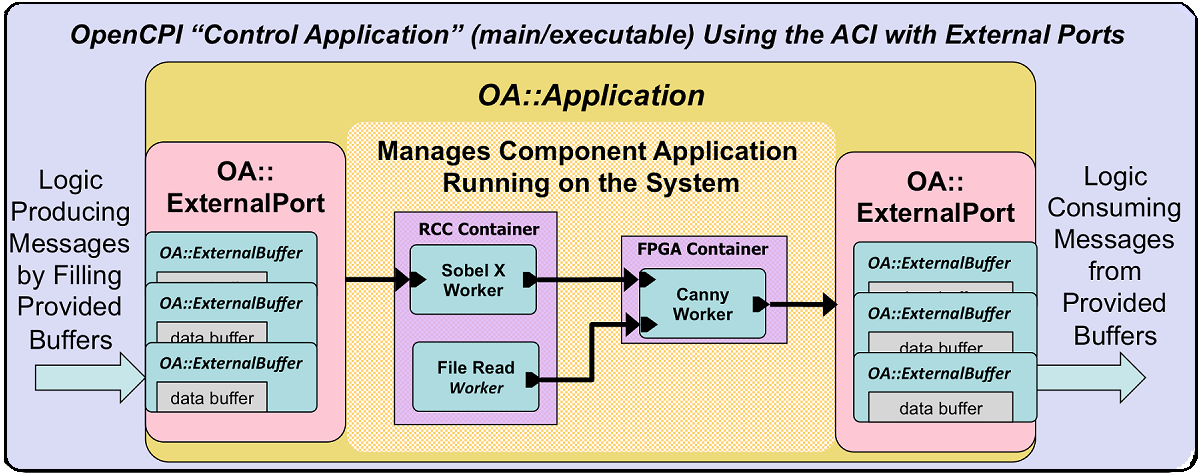
\includegraphics[width=\textwidth]{Relationships}
	\caption{External Ports and Applications}\hypertarget{fig:Relationships}{}
	\end{figure}
\subsection{Class OA::ExternalPort} This class represents a communication endpoint for the control-application itself, used to communicate with external ports of the application.  These objects are owned by the {OA::Application} object and should not be deleted directly.
\subsubsection{OA::Application::getBuffer Method}This method is used to retrieve the next available buffer of the port.  It returns a pointer to an OA::ExternalBuffer object, or NULL if there is no buffer available.  Thus it is a non-blocking I/O call.  The buffer objects encapsulate the actual raw data buffers and are owned by the OA::ExternalPort objects. \\

For external ports giving data to the application (connected to a worker input port inside the application), the returned buffer object manages a data buffer to fill with a message to send into the application.  For external ports taking data from the application, the returned buffer object manages a data buffer containing the next message to be received by the control-application.  When the control-application is done with the buffer, it calls the put method (when giving data) or the release method (when taking data). \\

In addition to returning a pointer to the buffer object, the getBuffer method also returns (as output arguments by reference), a pointer to its raw data buffer and the length of the message (when taking) or the length of the buffer (when giving).  These are convenience values that are attributes of the returned buffer object.  The data pointer returned by reference points to memory owned by the buffer object.\\

There are two overloaded getBuffer methods, for the two directions.  The first, for taking data by getting a buffer filled with a message, also returns the metadata for the message (opCode and endOfData) in separate by-reference output arguments.
\begin{ocpixml}
class ExternalPort {
 // Take data from app: get buffer filled with next message
    ExternalBuffer *getBuffer(uint8_t *&data,
                              uint32_t &length,
                              uint8_t &opCode,
                              bool &endOfData);
// Give data to app: get buffer to fill with next message
 ExternalBuffer *getBuffer(uint8_t *&data, uint32_t &length);
  };
\end{ocpixml} 
\subsubsection{OA::ExternalPort::endOfData Method} This method indicates that no more messages will be sent to the application on this external port.  It is only used when giving data.  This propagates an out-of-band indication across the connection to the worker port.  Note that this indication can also be made in the OA::ExternalBuffer::put() method below if the message being sent is the last message to be sent.  This latter method may be more efficient, since the out-of- band indication can be carried with the message, rather than by itself. 
\begin{ocpixml}  
class ExternalPort {
void endOfData();
 }; \end{ocpixml} 
\subsubsection{Class OA::ExternalBuffer}This class represents buffers attached to (and owned by) ExternalPort objects.They are returned (by pointer return value) from the OA::ExternalPort::getBuffer methods, and recycled back to the external port via the put method (when giving data to the application) or the release method (when taking data from the application).These objects encapsulate raw data buffers which are provided to the caller of the OA::ExternalPort::getBuffer methods via an output pointer argument, by reference.  Thus all buffering is managed by these objects, and pointers to the objects as well as to the internal raw data buffers are provided to callers.
\subsubsection{OA::ExternalBuffer::release Method} This is the method used to discard an input buffer (output from the application) after the message in it has been processed/consumed by the control-application. 
\begin{ocpixml}  
class ExternalBuffer {
    void release();
  };\end{ocpixml} 
A simple loop that prints 10 (text) messages (without blocking or yielding) might be:
for (unsigned n = 0; n < 10; ++n) 
\begin{ocpixml}  
{
    	OA::ExternalBuffer *b;
    	uint8_t *data, opcode;  size_t length;  bool end;
    	do b = port.getBuffer(data, length, opcode, end); while (!b);
   	printf (%u: .*s\n, opcode, (int)length, data);
   	b->release();
  }  \end{ocpixml} 
\subsubsection{OCPI::ExternalBuffer::put Method} This method is used to send an output buffer after it has been filled by the control-application.  The arguments specify the metadata associated with the message:\begin{itemize}
\item  the length in bytes of  message data
\item  the opcode of the message
\item  whether it is the last message to be sent
\end{itemize}If it is not known whether the message is the last to be sent at the time of the call, it can be sent without that indication, and the endOfData() method can be called on the ExternalPort object at a later time.\\

The declaration is: 
\begin{ocpixml}  
	class ExternalBuffer {
		void put(uint32_t length,
		uint8_t opCode = 0, 
		bool endOfData = false);
  };\end{ocpixml} 
A simple loop that fills/sends 10 (text) messages (without blocking or yielding) might be:
  for (unsigned n = 0; n < 10; ++n) 
\begin{ocpixml}  
{
   OA::ExternalBuffer *b;
    uint8_t *data;  size_t length;
    do b = port.getBuffer(data, length); while (!b);
    snprintf(data, length, Message number %n, n);
    b->put(strlen(data), 0);
  }
  port.endOfData();  \end{ocpixml} 
\subsubsection{Class OA::Property} This class represents a runtime accessor for a property.  They are normally created with automatic storage (on the stack) and simply cache the necessary information to very efficiently read or write property values.  The control-application that uses this class is responsible for creating and deleting the objects, although typical usage is automatic instances that are automatically deleted.
\subsubsection{OA::Property::Property Constructor Method} This constructor initializes the Property object such that it is specific to the application and specific to a single named property of that application.  
\begin{ocpixml}  
  class Property {
  Property(Application &app, const char *name);
  }; \end{ocpixml} 

The name argument specifies the property the same as the getProperty method in the application class described above.  Typical usage would be:
\begin{ocpixml}  
  {
    OA::Application app(myapp.xml);
    app.initialize();
    OA::Property freq(w, frequency), peak(w, peak);
    app.start();
    freq.setFloatValue(5.4);        // set this during execution
    float p = peak.getFloatValue(); // get this during execution
    app.wait();
  }\end{ocpixml} 
The \emph{set} and \emph{get} methods are all strictly typed.  They cannot be overloaded since overloading of integral types in C++ does not prevent truncation.
This same class is used in the more detailed ACI classes described below. In particular, there is another constructor for this class based on a Worker object:  \begin{ocpixml}  
class Property {
    Property(Worker & worker, const char *name);
  };\end{ocpixml} 
Beyond the fact that it is based on a worker rather than an application, the constructed property object is used with all the same methods.
\subsubsection{OA::Property::set (Type)Value Methods}There is a \emph{set} method for each property scalar data type.  The set methods are strongly typed and individually named to avoid the unintended consequences of numerical type conversions of the C++ language.  If the wrong set method is used for a property (e.g. setULong for a property whose type of Float), an exception is thrown.  If the string in setStringValue is longer than the worker property's maximum string length, an exception is thrown.
\begin{ocpixml}  
class Property {
  void setBoolValue(bool val);
  void setCharValue(int8_t val);
  void setDoubleValue(double val);
  void setFloatValue(float val);
  void setShortValue(int16_t val);
  void setLongValue(int32_t val);
  void setUCharValue(uint8_t val);
  void setULongValue(uint32_t val);
  void setUShortValue(uint16_t val);
  void setLongLongValue(int64_t val);
  void setULongLongValue(uint64_t val);
  void setStringValue(const char *string);
};\end{ocpixml} 
\subsubsection{OA::Property::get(Type)Value Methods} 
There is a \emph{get} method for each property data type. The get methods are strongly typed and individually named to avoid the unintended consequences of numerical type conversions of the C++ language.  If the wrong get method is used for a property e.g. getULong whose type of Float, an exception is thrown.  If the string buffer in getStringValue is not long enough to hold the worker property's current string value, an exception is thrown.  If there is an error accessing the workers property value, an exception is thrown. 
\begin{ocpixml}  
class Property {
  bool getBoolValue();
  int8_t getCharValue();
  double getDoubleValue();
  float getFloatValue();
  int16_t getShortValue();
  int32_t getLongValue();
  uint8_t getUCharValue();
  uint32_t getULongValue();
  uint16_t getUShortValue();
  int64_t getLongLongValue();
  uint64_t getULongLongValue();
  void getStringValue(char *string, unsigned length);
}; \end{ocpixml} 
\subsubsection{OA::Property::set(Type)SequenceValue Methods} 
There is a set sequence method for each property data. The set sequence methods are strongly typed and individually named. If the wrong set sequence method is used for a property e.g. setULongSequence for a property whose type of Float, an exception is thrown. If any of the strings in setStringValueSequence is longer than the property's maximum string length, an exception is thrown. It the number of items in the provided sequence is greater than the maximum sequence or array length of the property, an exception is thrown. If there is an error accessing the property value, an exception is thrown.
\begin{ocpixml}  
class Property {
  void
  setBoolSequenceValue(bool *vals, unsigned n),
  setCharSequenceValue(int8_t *vals, unsigned n),
  setDoubleSequenceValue(double *vals, unsigned n),
  setFloatSequenceValue(float *vals, unsigned n),
  setShortSequenceValue(int16_t *vals, unsigned n),
  setLongSequenceValue(int32_t *vals, unsigned n),
  setUCharSequenceValue(uint8_t *vals, unsigned n),
  setULongSequenceValue(uint32_t *vals, unsigned n),
  setUShortSequenceValue(uint16_t *vals, unsigned n),
  setLongLongSequenceValue(int64_t *vals, unsigned n),
  setULongLongSequenceValue(uint64_t *vals, unsigned n),
  setStringSequenceValue(const char **string, unsigned n);
}; \end{ocpixml} 
\subsubsection {OA::Property::get(Type)SequenceValue methods} 
There is a "get sequence" method for each scalar data type. The get sequence methods are strongly typed and individually named.  If the wrong get sequence method is used for a property e.g. getULongSequenceValue for a property whose type of Float, an exception is thrown. If there is an error accessing the workers property value, an exception is thrown. The first argument, vals, points to an array where the values will be placed.  The second argument, n, is the space available provided by the caller.  If there is not enough room in the array, an exception is thrown.  The return value is the number of elements returned in the array.
\begin{ocpixml}  
class Property {
 unsigned
  getBoolSequenceValue(bool *vals, unsigned n),
  getCharSequenceValue(int8_t *vals, unsigned n),
  getDoubleSequenceValue(double *vals, unsigned n),
  getFloatSequenceValue(float *vals, unsigned n),
  getShortSequenceValue(int16_t *vals, unsigned n),
  getLongSequenceValue(int32_t *vals, unsigned n),
  getUCharSequenceValue(uint8_t *vals, unsigned n),
  getULongSequenceValue(uint32_t *vals, unsigned n),
  getUShortSequenceValue(uint16_t *vals, unsigned n),
  getLongLongSequenceValue(int64_t *vals, unsigned n),
  getULongLongSequenceValue(uint64_t *vals, unsigned n),
  getStringSequenceValue(const char **string, unsigned n,
  char *buf, unsigned maxStringSpace);
};\end{ocpixml} 

For getStringSequenceValue, the first argument is an array of pointers provided by the caller, whose length is n.  These pointers will point to the returned strings.  The buf argument is space for the returned strings to be stored, whose length is indicated by the maxStringSpace argument.  If maxStringSpace is insufficient to store all the strings (each with null termination), an exception will be thrown.
\subsubsection{Class OA::PValue: Named and Typed Parameters}\hypertarget{Class OA::PValue: named and typed parameters}{Class OA::PValue: named and typed parameters} This class represents a strongly typed name/value pair, and is always used as a member of a null-terminated array of such objects.  Its usage is typically to provide a pointer to an array of PValue structures, usually statically initialized.  There are derived classes (of OA::PValue) for each supported data type, which is the same set of types supported for component properties in the OCS. For each supported scalar data type, the name of the derived class is OA::P $<$type$>$, where $<$type$>$ can be any of:
\begin{verbatim} Bool, Char, Double, Float, Short, Long, UChar, ULong, UShort, LongLong, ULongLong, or String 
The corresponding C++ data types are:
bool, char, double, float, int16_t, int32_t, uint8_t, 
uint32_t, uint16_t,int64_t, uint64_t, char *\end{verbatim} 

Common usage for static initialization is to declare a PValue array and initialize it with typed values and terminate the array with the symbol PVEnd, which is a value with no name, e.g.:
\begin{ocpixml}
PValue pvlist[] = {
  PVULong("bufferCount", 7),
  PVString("xferRole", active),
  PVULong("bufferSize", 1024),
  PVEnd };
\end{ocpixml}
Note that OA::PValue objects are used to provide named and typed parameters to the ACI, and are in fact unrelated to component properties except they share data types.
\subsubsection{Building ACI programs} Programs using the ACI are normally built in the context of OpenCPI projects, \hyperlink{Applications in projects}{(see Applications in Projects)} in which case the compilation and link commands are provided by OpenCPI.  When the ACI is used outside OpenCPI projects, presumably in the context of other software libraries or executables, the OpenCPI CDK must still be installed.\\

The make file fragment ocpisetup.mk (from the include subdirectory of the CDK installation) can be included or examined to determine the correct values of gnumakevariables for use outside OpenCPI projects.  In particular:
\begin{itemize}
\item The include file search path must include the directory defined in {OCPI\_INC\_DIR}
\item  External OpenCPI symbols in the executable must be available to dynamically\\
loaded libraries using linker options defined in \emph{OCPI\_EXPORT\_DYNAMIC}
\item The link-time library search path (usually using -L options) must include the\\
directory in \emph{OCPI\_LIB\_DIR}
\item The OpenCPI framework libraries found in the \emph{OCPI\_API\_LIBS} variable must be\\
 included in the link command, typically using: \$ (OCPI\_API\_LIBS :\%$=$-locpi\_\%)
\item The OpenCPI prerequisite libraries found in the \emph{OCPI\_PREREQUISITE\_LIBS}\\
 must be included as \emph{static} libraries using, e.g.:
\begin{verbatim}$ (foreach 1, $ (OCPI_PREREQUISITES_LIBS), 
/opt/opencpi/prerequisites/$1/linux-c7-x86_64/lib/lib$1.a)\end{verbatim}
\end{itemize}
Building ACI programs for embedded systems outside of OpenCPI projects is not explicitly supported.

\subsection{Using the ACI with Python}\hypertarget{Using the ACI with Python}{}
\emph{This feature is preliminary and subject to change.}\\
If the program using the ACI is written in Python, the ACI can be used directly by importing the OcpiApi module. This module serves as the namespace for the Python ACI, much like the OCPI::API C++ namespace.  Thus a typical initial python code might be: import OcpiApi as OA app = OA.Application('myapp.xml'). The same object classes and methods described for C++ are available in Python, with the following rules and exceptions. Methods that have by-reference output arguments in C++ return a tuple in Python consisting of the normal return value followed by all the by-reference output arguments described for C++. \\
For example, the getBuffer method of the xternalPort class is defined in C++ as: ExternalBuffer *getBuffer(uint8\_t *\&data, uint32\_t \&length); A use of this method in C++ would look like:\begin{verbatim}
uint8_t *data;
uint32_t length;
ExternalBuffer *buffer = port.getBuffer(data, length);
In python this would be: buffer, data, length = port.getBuffer() \end{verbatim} To access (import) the \emph{OcpiApi} package, the files\emph{\_OcpiApi.so and OcpiApi.py} should be either in the PYTHONPATH, the current working directory, or under the standard install path of python under the \emph{site-packages} directory.  When using the RPM installation, this is done automatically.
\section{Using Remote Containers: Network-Connected Processors}\label{sec:Using remote containers} \emph{This feature is preliminary and subject to change.}\\
When an application is run, containers are found on the local system where workers (based on artifacts) may execute.  The set of containers considered are those that are part of, or directly attached to, the local system.  This includes RCC (software)containers based on the local CPU, and FPGAs attached to the system's bus or fabric such as PCI Express or the local interconnect between CPU and FPGA on Zynq SoCs. \\

The {remote containers} feature adds containers available in other systems on the network to the set of containers considered for execution.  Remote containers are containers offered for use by these other network-based systems.\\

An OpenCPI system may offer its containers to other systems for use as remote containers by running the \emph{ocpiserve} command.  This command, when run on a system says:  make my local containers available for use by other systems which act as network clients.  The ocpiserve command runs a "container server" serving up local containers as remotely accessible containers to network clients. There are several reasons for remote containers:
\begin{itemize}
\item  Scaling the available resources by using all the containers on a collection of network-connected systems (e.g. clusters, multiple radios)
\item  Heterogeneous testing, control, experimentation by allowing the application control and testing client to use and control many disparate platforms
\item  Support containers only controllable via networks like plug-in processor cards controllable via network over backplane signals, or virtual machines running other OSs or licensed simulators
\item  Support minimally configured embedded server nodes which only require ocpiserve to run and nothing else (minimal configuration and footprint)
\end{itemize}
\subsection{Using ocpirun with Remote Containers} While ocpiserve enables containers to be offered by a remote system,  its containers are only used when clients are similarly enabled to discover and use them.  The ocpirun command has two options for this purpose. The -R (--remote) option tells ocpirun to discover and use remote containers.  The discovery function uses a multicast technique to find the systems running ocpiserve, and retrieve from them the list of available containers on each such system. Similarly, the -S (--server) option to ocpirun specifies the IP address of a specific system where ocpiserve is expected to be running.  This option avoids any necessity of discovery or multicast, but requires a manual method to obtain the IP address of the server system and provide that address to the ocpirun command. \\

The command: ocpirun -R -C runs ocpirun simply to list available containers, including any discovered remote ones. Similarly, there is a -d (-- discoverable) option to ocpiserve that says:  make ocpiserve discoverable via multicast.  This enables clients using the -R option to find the server. Without the -d (-- discoverable) option, the ocpiserve command must be contacted using its explicit IP address (using the -S option to ocpirun). The ocpiserve command is fully described below.
\subsection{ACI functions for using remote containers}
If the client system is using the ACI, then there are two functions that serve purposes similar to the -R and -S options to ocpirun. The function:  
voidOA::enableServerDiscovery(); \\
is the ACI equivalent to the ocpirun -R option, and enables remote container discovery.The function: 
void OA::userServer(const char *server);\\
is the ACI equivalent to the ocpirun -S option. And the function: bool OA::isServerSupportAvailable(); is a simple function to use to determine whether remote container support is enabled in the current environment.  This function can be called early in the ACI program to decide whether the other two should be called at all.  it essentially indicates whether the remote container driver is loaded via being specified in the system.xml file.
\subsection{Environment Variables for Using Remote Containers} 
The OCPI\_ENABLE\_REMOTE\_DISCOVERY variable can be set to 1 to enable the multicast discovery of servers running ocpiserve.  There are also environment variables that specify which remote servers to contact (independent of multicast discovery).  All these variables may be applied to either ocpirun or ACI programs, as well as unit testing.\\

The OCPI\_SERVER\_ADDRESSES environment variable may contain a space-separated list of IP addresses of servers to contact, and the OCPI\_SERVER\_ADDRESSES\_FILE environment variable may contain a filename containing server IP addresses, one per line.  Using these variables enables the use of multiple remote systems' containers for any ocpirun, ACI or unit test execution.\\

The OCPI\_SERVER\_ADDRESSES\_FILE variable can sometimes be used when the client and server both have the same file system mounted since the ocpiserve command can be told to put its address(es) into a named file (see below).  This is a tradeoff between the overhead and complexity of having a common mounted file system (e.g. when the server has an NFS mount to the client or vice versa), vs. the need to know the server's IP address, which could be dynamically determined by DHCP.\\

If you cannot use server discovery and already have a common NFS mounted directory, \\
using OCPI\_SERVER\_ADDRESSES\_FILE is a convenient way to avoid knowing or typing or copy-pasting IP addresses.  If you cannot use discovery and do not want or have a common mounted file system, using OCPI\_SERVER\_ADDRESSES on the client side may be best.  The ocpiserve -v option causes ocpiserve to print out its IP addresses.
\subsection{Using ocpiserve to Offer Remote Containers to Clients}
The ocpiserve command offers local containers to remote clients.  When it starts, ocpiserve discovers all local network interfaces and prepares to be contacted by clients on all of them. When given the {-d (--discoverable)} option, it also prepares to receive multicast queries from clients on all interfaces.  It is a fully multi-homed server, using all interfaces for normal usage (via TCP) and discovery (via multicast UDP). \\

The ocpiserve command does not use the {OCPI\_LIBRARY\_PATH} environment variable since the client-server protocol used automatically downloads (from client to server) each artifact needed by any application using these remote containers.  This automatic artifact downloading operates as a cache. When any client requests execution on any of ocpiserve's containers, they also indicate which artifacts should be used in each container. If these artifacts have been previously downloaded, they are reused.  If not, they are downloaded from client to server.The ocpiserve command maintains this cache in a directory called artifacts (unless overridden by an option-see below). The artifact cache is normally maintained after ocpiserve exists (usually via control-C).  An option indicates whether it should be removed when ocpiserve exits.\\
\newpage
\begin{table}[h!]
\caption{Options to ocpirun}
\renewcommand*{\arraystretch}{2.5}
\begin{tabular}[c] { |c|c|c|p{11cm}|}
\hline \emph{Name} & \emph{Letter} & \emph{Datatype} & \emph{Description}\\
\hline
verbose &	v &	Bool &	Print status and progress as ocpiserve executes\\
\hline 
log-level & l &	UChar &	Set the logging level during execution\\
\hline
 directory &	D	& String &	The name of the directory to use for caching downloaded artifacts.  The default is artifacts.\\
\hline 
processors &	n &	UShort & How many local RCC containers to create and serve.  The default is 1 (one).\\
\hline 
remove &	r & Bool & Remove artifact cache when ocpiserve exits.\\
\hline 
port	& p	& UShort &	The TCP port to be used for server ports.  The default is dynamically assigned port numbers.\\
\hline 
discoverable	& d	& Bool & Whether to become discoverable via UDP multicast.\\
\hline 
addresses &	a &	String &	File name for a file where ocpiserve will write all its TCP addresses.\\
\hline
loopback &	L	& Bool & Enable/add discovery on the local loopback subnet.\\
\hline 
onlyloopback &	O	& Bool	& Allow discovery only on the local loopback subnet.\\
\hline
\end{tabular}
\end{table}
Note that some option must be present otherwise ocpiserve will simply print a help message.  A typical execution is: ocpiserve -v -d.
\subsection{Remote Containers Setup Requirements} In order for remote containers to be fully enabled several setup requirements must be met, both on the client side and on the server side.
\subsubsection{Client Side Remote Container Setup Requirements}Client systems must be enabled for remote containers.  The first requirement is that the remote container OpenCPI driver must be loaded, which is specified in the system.xml file for the client system.E.g. the load attribute of the remote container driver must be set to one: \begin{ocpixml}
<opencpi>
   	<container>
    	<rcc load='1'/>
    	<remoteload='1'/>
   	...
    	</container>
   	 ...
</opencpi>\end{ocpixml}
The second requirement to enable clients to automatically discover servers via multicast UDP, is to provide a proper multicast route to the local network interface on the client system.  This is normally accomplished by a command such as:\begin{verbatim}route -n add -net 224.0.0.0 netmask 240.0.0.0 dev enp2s0. \end{verbatim} This assumes the normal default network interface for the client is enp2s0.
\subsubsection{Server Side Remote Container Setup Requirements} 
On the server side, the ocpiserve executable must be present and there should be enough disk space to hold the artifact cache. To allow the server to be discovered, its local firewall must allow inbound UDP multicast packets from the local network or at least selected clients.  To open the firewall to local network traffic the following command can be used: firewall-cmd --zone=trusted --add-interface=eth0. Of course more fine-grained permissions may be appropriate.
\section{Preparing HDL Assemblies for Use by Applications} \label{Preparing HDL Assemblies for Use by Applications}   
Developing HDL component implementations (workers) for FPGAs is out of scope for this application development guide -that process is fully described in the \emph{OpenCPI Component Development Guide} at \url{github.io/opencpi/opencpi/raw/2018.Q1/doc/pdf}.  Utilizing FPGAs in OpenCPI requires that component libraries, with built/compiled HDL/FPGA workers, be supplied for applications to use FPGAs.\\

HDL assemblies are the way compiled HDL workers (in built component libraries) are transformed into the artifacts necessary to execute applications that use workers executing on FPGAs.  The steps to using FPGAs with OpenCPI are:
\begin{enumerate}
\item HDL workers are written in an HDL (hardware description language), typically VHDL.
\item HDL workers are built/compiled for a specific type of FPGA (e.g. Xilinx Zynq or Altera Stratix4)
\item HDL assemblies are defined in simple XML files as a set of connected HDL workers that can act as a proper subset of an application.
\item HDL assemblies are converted into ready-to-execute artifacts by a build process that incorporates the built/compiled HDL workers into a bitstream file targeting a particular FPGA platform.
\end{enumerate}
Steps 1 and 2 are performed by HDL component developers who create libraries of HDL workers compiled for a variety of targeted FPGA devices.\\

Steps 3 and 4 \emph{do not require VHDL coding or specific knowledge of or interaction with FPGA tools}, but the FPGA development tools (as well as the CDK) are required to be installed. \\

Step 4 is more complex when the application is accessing I/O devices directly attached to the FPGA, but still requires no VHDL coding nor vendor tools knowledge.\\

Thus HDL assemblies are in a middle ground between HDL worker development and application execution.  Once artifacts are produced from HDL assemblies, neither the CDK nor the FPGA build tools are required. A set of artifacts based on HDL assemblies and built for some HDL platforms, acts as a runtime library for using FPGAs to support executing applications. \\

Except under unusual conditions (e.g. when the HDL assembly does not fit into the targeted FPGA device), building FPGA artifacts using HDL assemblies can be considered part of application development, and not component development.\\

Creating HDL assemblies in projects is described in the section \hyperlink{HDL Assemblies in Projects} {HDL Assemblies in Projects}. Building HDL assemblies outside of projects is not explicitly supported. \\

The section, \emph{HDL Assemblies for Creating Bitstreams in the OpenCPI HDL Development Guide}, describe steps 3 and 4 in detail.
\section{Developing Applications in OpenCPI Projects}\hypertarget{Developing applications}Applications are typically XML files (OASs) that rely on the existence of existing artifacts via OCPI\_LIBRARY\_PATH.  They may also be C++ or Python main programs using the ACI. Applications may also be created as part of an OpenCPI project containing other OpenCPI assets such as components, workers, primitive libraries, etc. In OpenCPI a project represents a work area in which a variety of assets are created and developed.  Projects can contain all types of OpenCPI assets that are described in this document or in others.\\

A project can contain: \begin{itemize}
\item Component libraries with specs and workers (described in the \emph{Component Development Guide})
\item Applications whether simple XML or using the ACI \emph{(described here)}
\item HDL primitives and assemblies (described in the \emph{HDL Development Guide})
\item HDL devices, cards, slots (described in the \emph{HDL Development Guide})
\item Platform support assets (described in the\emph{Platform Development Guide})\end{itemize}

A project uses a standardized directory structure that holds the various OpenCPI assets in source code form, along with other files that describe how they are built.  The project structure provides a means to co-develop a collection of assets which may have a logical relationship or be created for a specific overall application.  Projects may depend on other projects when assets from other projects are needed.\\

All of the assets in a project have a package ID, which all normally share a project-level package prefix. When an OpenCPI application is developed in a project, an IDE or the ocpidev command line tool is used to manage the project and the assets inside it.  Even if the project contains only applications, there are advantages to putting applications into OpenCPI projects, especially during development and especially for ACI-based applications.  The ocpidev tool is described next. Discussing any IDE for this purpose is out of scope for this document.\\

Projects are for development.  When an OpenCPI application is deployed on a runtime-only non-development system, projects are not used.  Deploying applications and the various files they depend on (e.g. OAS files, ACI executables, artifacts, ocpirun), is described in the \hyperlink{Developing applications} {Deploying Applications in a Runtime Environment} section below.
\subsection{The ocpidev Tool as Used for OpenCPI Applications in Projects}The ocpidev command is fully described and documented in the CDG, but for pure application users (that are not developing other asset types), the small necessary subset of this tool's functionality is described here.  Projects are created with the command:\begin{ocpixml}
% ocpidev [options] create project <name>
\end{ocpixml}

This creates a project in a directory $<$name$>$ which must be a name without slashes. The project directory is created under the current working directory where ocpidev is executed.The -d $<$directory$>$ option can be used to create the project's directory under a different directory. The options available during project creation are:
\begin{table}[h!]
\caption{Options for ocpirun during Project Creation}
\renewcommand*{\arraystretch}{2.5}
\begin{tabular}[c] {|c|c|c|p{12cm}|}
\hline
\emph{Option} & \emph{Value?} & \emph{Default} & \emph{Description}\\
\hline
-v	&	no	&	{} & Be verbose, describing what is happening in more detail\\
\hline 
--help	& no &	{} & Show message explaining how ocpidev can be used\\
\hline
 -d	&	yes	& {}	& Specify the directory in which this command should be performed, analogous to the -C option in the POSIX make command\\
\hline
 -D	&	yes & {} &	Specify a project (using its package-ID) that this project depends on\\
\hline 
-K &	yes	& local	& Specify the package ID when creating a project\\
\hline
\end{tabular}
\end{table}
\\
The -D option is useful to specify other projects that the assets in this project depend on, such as projects that may contain component libraries.  The -K option is only needed when the project will be globally published and requires a globally unique name. Projects are deleted using the  command:\begin{ocpixml}
{% ocpidev [options] delete application <name>}. 
\end{ocpixml}

When using projects only for applications only two types of assets are created in the project: applications and HDL assemblies.
\subsection{Applications in Projects}\hypertarget{Applications in projects}Applications in projects live in the applications/ subdirectory of the project and are either XML applications, based on an OAS file, or ACI-based C++ programs.  XML applications can simply be OAS files in the applications/subdirectory, or be in a directory of their own, also under applications.  ACI-based applications are always in their own directory. Applications are created in projects by executing this command in a project's directory or in its applications/subdirectory:
\begin{ocpixml}
{% ocpidev [options] create application <name>}. 
\end{ocpixml}

\begin{table}[h!]
\caption{Options for ocpirun when Creating Applications}
\renewcommand*{\arraystretch}{2.5}
\begin{tabular}[c] {|c|c|c|p{12cm}|}
\hline
\emph{Option} & \emph{Value?} & \emph{Default} & \emph{Description}\\
\hline
-v	&	no	&	{} & Be verbose, describing what is happening in more detail\\
\hline 
-X	& no &	{} & The application will be a simple XML OAS file in the
applications/directory of the project named \emph{$<$name$>$.xml}\\
\hline 
-x	& no &	{} & The application will be an XML application file in its own directory, in \emph{applications/name/name.xml}\\
\hline
\end{tabular}
\end{table}

The -X or -x options specify an XML application, the latter in its own directory.  In these cases an empty OAS file is created with the indicated name and can then be edited as necessary to create the application.\\

Without the -X or -x  options, an ACI C++ application is created in its own directory under the applications directory with the indicated name in a file named $<$name$>$.cc, containing the main program.\\

When an application is created in its own directory (either XML or ACI C++) a default Makefile is created in that directory.  Placing an application in its own directory allows customizations in the associated Makefile for options, and the inclusions of test or data files or even other make targets.\\

The Makefile in the top level applications/directory will build (for ACI-based C++ applications), and execute all applications.  If only a subset of the applications should be built or executed, or if they must be built or executed in a particular order, the Applications variable may be set in this Makefile to contain a list of the applications to be used and the order in which they are built and/or used, e.g.:
\begin{ocpixml}
Applications = myapp1 myapp3 # do not use myapp2 for now. 
\end{ocpixml}

Even when an application is excluded from the Applications variable, it is still possible to manually enter its directory and build or run there. To delete applications, the following command is used.  The same options allowed for creating an application are valid for deleting one.
\begin{ocpixml}
ocpidev [options] delete application <name>
\end{ocpixml}
The default make goal for the applications directory is to build all ACI applications. The run goal is used to execute all applications, either pure XML or ACI.
\subsubsection{Building Applications in Projects} ACI-based applications are built in their own directories using the ocpidev command. From a project's top level directory or the applications subdirectory, a specific application can be built using the command: 
\begin{ocpixml}
% ocpidev [options] build application <name> 
\end{ocpixml}

To build all applications in a project, you can issue the following command either in the project's directory or in its applications subdirectory: \begin{ocpixml}
% ocpidev build applications 
\end{ocpixml} 
From the application's directory itself, you can simply use:
\begin{ocpixml}
% ocpidev build 
\end{ocpixml}

With no target platform specified, the executable is built to run on the development system itself.  To build for other software platforms, you can use the \emph{--rcc-platform} option (multiple times if desired).\\
E.g., for the ZedBoard embedded platform, the software platform name for the embedded linux is something like xilinx13\_3. Thus to build ACI program for that system would be:
\begin{ocpixml}
% ocpidev --rcc-platform xilinx13_3 build 
\end{ocpixml}
To build the application for a software (RCC) platform associated with a particular HDL platform, you can use the option --hdl-rcc-platform, which essentially adds the RCC platform associated with the specified HDL platform to the platforms to build.  Not all HDL platforms have a specific associated RCC platforms, but SoC platforms like Zynq usually do, since there is an FPGA side and a GPP CPU side to one chip.\\

All executables are created in subdirectories named target-$<$platform$>$, so executables for multiple different platforms can coexist. 
\subsubsection{Application Makefiles} The Makefile in an ACI application's directory in a project is normally used as it is initially created by ocpidev. Several make variables can be set in this file to customize the application's build or execution behavior.\\

The OcpiApp variable can be set to indicate the file name of the application's main C++ file.  Normally this defaults to the name of the application's directory which is the name of the application given to ocpidev when it was created.  The OcpiApps variable can be specified to build more than one executable in this application's directory.  OcpiApps provides file names (without suffix) of other files that should be built as separate executables. \\
The OcpiAppNoRun variable, when not empty, prevents the Makefile from allowing the application to execute using the run goal (or ocpidev run verb), whether invoked.
\subsubsection{Executing Applications in Projects} Simple OAS XML applications may be run directly using the ocpirun command.  All applications in a project may be run in sequence using the command:

\begin{ocpixml}
% ocpidev run applications
\end{ocpixml}
from a project directory or its applications/ subdirectory.  
In the applications/ directory, only this command is necessary to run all applications:
\begin{ocpixml}
% ocpidev run
\end{ocpixml}
These will run all applications, one after the other, with no arguments specified.   To run a particular ACI application, you can either run ocpidev run in the application's directory, or, from the project or applications/ directory, you can use:
\begin{ocpixml}
% ocpidev run application<appname>
\end{ocpixml}
To run a specific XML application, ocpidev cannot be used (yet), but you can use:
\begin{ocpixml}
% make run Applications=<foo.xml>
\end{ocpixml}
Running all the applications in a project with default arguments is normally used for test purposes.\\

To provide arguments to applications, these Makefile variables may be set, either in Makefiles or on the make command line.\\
\newpage
\begin{table}[h!]
\caption{Make Variables for Running Applications}\label{Make Variables for Running Applications}
\renewcommand*{\arraystretch}{2.5}
\begin{tabular} { |c|p{12cm}|}
\hline
\emph{Makefile Variable} & \emph{Description}\\
\hline
OcpiRunBefore &	Arguments to insert before the ACI executable or ocpirun, such as environment settings or prefix commands like \emph{time} or \emph{valgrind}.\\ 
\hline 
OcpiRunArgs & Arguments to insert immediately after the ACI executable or \emph{ocpirun}, such as ocpirun options like \emph{-v or -m -or -p}\\ 
\hline 
OcpiRunAfter	& Arguments to insert at the end of the execution command line\\ 
\hline 
OcpiRunBefore\_$<$app$>$ & Like OcpiRunBefore, but only for the \emph{$<$app$>$} application\\ 
\hline 
OcpiRunArgs\_$<$app$>$ &	Like OcpiRunBefore, but only for the \emph{$<$app$>$} application\\
\hline 
OcpiRunAfter\_$<$app$>$ & Like OcpiRunBefore, but only for the \emph{$<$app$>$} application\\ 
\hline
\end{tabular}
\end{table}
For applications other than simple OAS XML applications without their own directory, the application's own Makefile may be customized using these variables. For XML applications, these variables are applied using the following pattern:
\begin{ocpixml}
<OcpiRunBefore> ocpirun <OcpiRunArgs> <xml-OAS-file> <OcpiRunAfter>\end{ocpixml}
For ACI C++ applications, the pattern is:
\begin{ocpixml}
<OcpiRunBefore> <executable> <OcpiRunArgs> <OcpiRunAfter>\end{ocpixml}
\subsection{HDL Assemblies in Projects}\hypertarget{HDL Assemblies in Projects} HDL assemblies may also be created in projects, using the command: 
\begin{ocpixml}
% ocpidev create hdl assembly <name>
\end{ocpixml}
Within a project, HDL assemblies are created in the hdl/assemblies/directory in the project.  Similar to applications, that directory has a standard Makefile and it can contain a setting of the Assemblies variable when the default behavior, of all assemblies being built in alphabetical order, is not desired. \\

Each assembly is created as an XML file in its own directory.  Thus creating the HDLassembly whose name is myassy, would create the myassy.xml file in the hdl/assemblies/myassy directory. After editing this file to describe the required worker instances and connections, artifacts based on this assembly can be created using the ocpidev build command in that assembly's directory or for building all the assemblies in the project, the ocpidev build hdl assemblies command may be issued from the project or hdl/assemblies directory.\\

The resulting FPGA artifact files, with the suffix.bitz, are created in target-specific directories with the prefix container-, created under the assembly's directory.
Details about this artifact building process are in the \emph{OpenCPI HDL Development Guide}. \\

HDL assemblies may be deleted using this command:
\begin{ocpixml}
% ocpidev delete hdl assembly <name>
\end{ocpixml} 
Once the HDL assemblies are built, resulting in the .bitz artifact files, applications can use them as long as they are accessible using the OCPI\_LIBRARY\_PATH environment variable.
\section{Deploying Applications in a Runtime Environment}\label{Deploying Applications in a Runtime Environment}OpenCPI applications require a small set of required dependencies during execution,which is considerably smaller than the requirements for OpenCPI development, which requires the installation of the OpenCPI Component Development Kit (CDK).  While the installation requirements and procedures are described in full in the \emph{OpenCPI Installation Guide}, the essential requirements required to support application execution are described here.\\

The basic requirements are to have the executable (ocpirun or a custom ACI C++ program), as well as the artifacts for the workers used during execution.  The executable can use whatever artifacts are available, as built for the available processing resources on the system.  By limiting the artifacts available (accessed via the\emph{OCPI\_LIBRARY\_PATH} environment variable setting), the system requirements are reduced to the minimum. \\

Beyond these two important elements (executables and artifacts), there are several dynamically loaded and used drivers, depending on which hardware resources are enabled for OpenCPI to use during execution.  There is a Linux kernel module that is loaded using the \emph{ocpidriver} command line tool.  There are user-mode drivers that are loaded according to a system configuration file, at \emph{/opt/opencpi/system.xml}, or a location indicated by the \emph{OCPI\_SYSTEM\_CONFIG} environment variable.\\
All of these drivers are optional, and used based on the hardware needed by OpenCPI application execution. \\

The following table lists the drivers and their use cases.\\
\begin{table}[h!]
\caption{Loadable Drivers for OpenCPI Execution}\label{Loadable Drivers for OpenCPI Execution}
\renewcommand*{\arraystretch}{2.5}
\begin{tabular} { |c|p{12cm}|}
\hline
\emph{Driver} & \emph{Required For:}\\
\hline
Kernel Module &	Access to DMA devices on the system bus.  E.g. FPGA PCIe cards in slots on the system's motherboard, or Zynq systems using the FPGA subsystem.  Loading this driver requires root/sudo privileges.
Loaded using the ocpidriver command.\\ 
\hline
RCC Container Driver & Execution of RCC/Software workers.  Indicated in system.xml\\ 
\hline 
HDL Container Driver &	Execution of HDL/FPGA workers (in hardware or in simulators).Indicated in system.xml\\
\hline 
DMA Transport Driver &	Data plane transport between software containers and DMA devices, e.g. FPGA containers.  Requires the kernel module to be loaded prior to execution.  Indicated in system.xml.\\ 
\hline 
PIO Transport Driver	& Data plane transport for software containers using shared memory.  Indicated in system.xml\\ 
\hline 
Socket Transport Driver &	Data plane transport for containers using network sockets.  Indicated in system.xml.  Required by HDL simulators and remote containers.\\ 
\hline
\end{tabular}
\end{table}

In addition to the executables, artifacts, and optionally loaded drivers, there are a small number of utility scripts (such as ocpidriver), support files (\/opt/opencpi/system.xml), and utility commands (which includes ocpirun) that are typically included in a runtime-installation.  Installation packages are generally prepared for a particular runtime environment.\\

For some hardware and software configurations, third party software is required for execution. Example is that for execution on FPGA boards that require dynamic JTAG loading of FPGA configuration files (bitstreams), there are drivers and utilities required from the FPGA vendors (Xilinx or Altera) that must be installed.\\
\newpage
\section{Execution Options Summary - Alphabetical}
\renewcommand*{\arraystretch}{2.5}
\begin{longtable} {| c| c| c |c|c|p{5cm}|}
\caption{Execution Options Summary-Alphabetical} \label{tab:long} \\
\hline \multicolumn{1}{|c|}{Name} & \multicolumn{1}{c|}{Letter} & \multicolumn{1}{c|}{Attribute}&\multicolumn{1}{c|}{PV Name}& \multicolumn{1}{c|}{Type}& \multicolumn{1}{l|}{Description} \\ \hline 
\endfirsthead
\multicolumn{6}{c}%
{{\bfseries \tablename\ \thetable{} -- continued from previous page}}\\
\hline 
\hline \multicolumn{1}{|c|}{Name} & \multicolumn{1}{c|}{Letter} & \multicolumn{1}{c|}{Attribute}&\multicolumn{1}{c|}{PV Name}& \multicolumn{1}{c|}{Type}& \multicolumn{1}{l|}{Description} \\ \hline  
\hline  
\endhead
\hline \multicolumn{6}{|c|}{{Continued on next page}} \\ \hline
\endfoot
\hline 
\endlastfoot
buffer-count & B & {} & buffer-count & String & Set the number of buffers for an instance port or an external port.
Name of file to be written\\ 
\hline  
buffer-size & Z & {} & buffer-size & String & Set the size of both ports of a connect for instance port or an external port\\ 
\hline 
container & c & {} & container & String & Specify the filename to write deployment decisions into, which can be used later using the deployment option\\ 
\hline 
deploy-out & {} & {} & {} & String & Specify the filename to write deployment decisions into, which can be used later using the deployment option\\ 
\hline 
deployment& {} &{}&{} &String &	Specify a deployment file, containing hardwired deployment decisions\\ 
\hline 
device & D	& {} & 	device & String	& Reserved for future use\\ 
\hline 
dump &	d &	{} & dump & Bool & Dump property values to stderr, before starting the application, and after it is done\\ 
\hline 
dump-file & {} & {} & dumpFile & String & Dump property values after the application is done, in a machine parseable format\\ 
\hline  
dump-platforms & M	& {}	& dump 
Platforms & Bool &	Dump property values for non-application workers before and after execution\\ 
\hline 
duration &	t & {} &{} & ULong & Run the application for a time duration in seconds if it doesn't finish earlier.\\ 
\hline 
file &	f	& {} &	file & 	String	& Connect an external port of the application to a file\\ 
\hline
hex & x	& {} & 	hex	& Bool	& When dumping property values, use hexadecimal when possible\\ 
\hline 
library-path & {} & {} &{} & String & Set the OCPI\_LIBRARY\_PATH\\
\hline
list&C&{}&{}&Bool&List available containers\\
\hline
list-artifacts&{}&{}&{}&Bool&List available artifacts for the target values provided using --target\\
\hline 
list-specs&{}&{}&{}&Bool&List available specs for the target values provided using --target.\\
\hline 
log-level & l&{}&{}&ULong & Set the logging level.\\
\hline
no-execute&{}&{}&{}&Bool&Figure out how to execute the application, but then don't actually execute.  Usually used with --deploy-out\\
\hline
model & m & {} & model & String & Specify the model for an instance\\
\hline
only-platforms & {} & {} & {} & Bool & When listing containers, actually only list platforms.\\
\hline
platform & P & {} & platform & String & Specify the platform for an instance\\
\hline
processors & n & {} & {} & ULong&Specify the number of RCC containers to create.\\
\hline
property & p & (element) & property & String & Instance-specific or application-level property value.\\
\hline
remote & R & {} & {}& Bool&Discover remote containers using Multicast UDP.\\
\hline
scale & N & {} & scale & Scale & Set the scale factor for an instance\\
\hline
selection & s & selection & selection & String & Set the selection expression  for an instance\\
\hline
server & S & {} & {} & String & Contact this server for remote containers\\
\hline 
sim-dir & s & {} & {} & String & Set the directory for simulation output\\
\hline 
sim-ticks & s & {} & {} & ULong & Set the directory for simulation output\\
\hline 
target & r & {} & {} & String & Set a target to use with list-artifacts or list-specs\\
\hline 
timeout & O & {} & {} & ULong & Set a timeout after which the application will be stopped and considered failed.\\
\hline 
transfer-role & O & {} & Transfer Role & String & Reserved\\
\hline
transport & T & transport & transport & String & Set the transport for a connection\\
\hline
uncached & U & {} & uncached & Bool & Dump properties without caching.\\
\hline
url&u&{}&url&String&Reserved\\
\hline
verbose & v &{}&verbose&Bool&Be verbose with messages\\
\hline
worker&w&worker&worker&String&Specify the worker for an instance.\\
\hline
\end{longtable}

\newpage
\section{Acronyms}
\begin{description}
\item[ACI] Application Control Interface 
\item[ARM] Advanced RISC Machine 
%\item[AV] ANGRYVIPER Team: sometimes used as prefix on ticket numbers within code
\item[AXI] Advanced eXtensible Interface 
\item[CBD] Component-Based Development
\item[BSP] Board Support Package 
\item[CDK] Component Development Kit
\item[CPU] Central Processing Unit 
\item[DSP] Digital Signal Processing or Digital Signal Processor 
\item[FPGA] Field Programmable Gate Array 
\item[GPGPU] General Purpose Graphics Processing Unit
\item[GPP] General Purpose Processor 
\item[GPU] Graphics Processing Unit 
\item[HDL] Hardware Description Language
\item[LVM] Logical Volume Manager 
\item[OAS] OpenCPI Application Specification
\item[OCL] OpenCL 
\item[OCS] OpenCPI Component Specification
\item[OHAD] OpenCPI HDL Assembly Description
\item[OpenCL] Open Computing Language
\item[OpenCPI] Open Component Portability Infrastructure
\item[OPS] OpenCPI Protocol Specification
\item[OSS] Open Source Software
\item[OWD] OpenCPI Worker Description
\item[PCI] Peripheral Component Interconnect
\item[PCIe] PCI-Express
\item[RCC] Resource Constrained C-Language: see RCC Authoring Model 
\item[RPM] RPM Package Manager
\item[UUT] Unit Under Test
\item[VHDL] VHSIC Hardware Description Language
\item[VM] Virtual Machine
\item[XML] eXtensible Markup Language 
\item[ZLM] Zero Length Message
\end{description}

\newpage
\section{Definitions}
\begin{description}[style=nextline]
\item[Adapter Worker]
Worker used when two connected workers are not connectable in some way due to different interface choices in the OWD.  Adapter workers are normally inserted automatically as needed, \textit{e.g.} between a \textit{worker} that has a 16-bit bus and one with a 32-bit one.

\item[Application]\hypertarget{application}{application}
In this context of Component-Based Development, an \textit{application} is a composition or assembly of \textit{components} that, as a whole, perform some useful function. The term ``application'' can also be an adjective to distinguish functions or code from infrastructure to support the execution of a component-based application, \textit{e.g.} a \textit{device worker} vs. an \textit{application worker}.

\item[Application Specification (OAS)]\hypertarget{OAS}{OAS}
An XML document that describes the collection of \textit{components} along with their interconnections and configuration properties in an OpenCPI \textit{application}.

\item[Application Worker]
Implementation of a function used in an \textit{application}, generally portable and hardware independent.

\item[Argument]
See \textit{operation argument}.

\item[Artifact]
A file containing executable code for one or more \textit{workers}  for a specific \textit{platform}.

\item[\emph{Authoring Model}] \hypertarget{authoring model}{authoring model}
One of several ways of creating \textit{component} implementations in a specific language using a specific API between the component and its execution environment.  Existing models include RCC and HDL\%, and OCL.

\item[AXI (Advanced eXtensible Interface)]
Industry-standard bus used by ARM processors.

\item[Board Support Package]
A \textit{project} that defines all items needed to enable OpenCPI on a given hardware and/or software \textit{platform}. This includes, but is not limited to, \textit{platform workers}, \textit{device workers}, configuration of software cross-compilers, etc.

\item[Component] \hypertarget{component}{component}
Interface ``contract'' that is specified by a \textit{component specification} and implemented by an \textit{application worker}.

\item[\emph{Component Application}] \hypertarget{component application}{component application}
A component application is a composition or assembly of components that as a whole perform some useful function.

\item[Component Development Kit]
Set of tools, scripts, documents, and libraries used for developing \textit{components} and \textit{workers} in \textit{projects}.

\item[Component Library]
Collection of \textit{component specifications} and \textit{workers} that can be built, exported, and installed to support \textit{applications}.

\item[Component Specification (OCS)]
An XML document that describes both \textit{configuration properties} and zero or more data interfaces (\textit{protocol specifications}) of a \textit{component}, establishing interface requirements for multiple implementations (\textit{workers}) in \textbf{any} authoring model.

\item [\emph{Configuration Properties}]\hypertarget{configuration properties}{configuration properties}
Named values of a \textit{worker} that may be read or written by \hyperlink{control software}{control software}. Their values indicate or control aspects of the \textit{worker}'s operation. Reading and writing these property values may or may not have side effects on the operation of the \textit{worker}. Configuration properties with side effects can be used for custom worker control. Each \textit{worker} may have its own, possibly unique, set of configuration properties. They may include hardware resources such registers, memory, and state.

\item[Containers]
OpenCPI infrastructure element that ``contains,'' manages, and executes a set of application \textit{workers}. Logically, the container ``surrounds'' the workers, mediating all interactions between the \textit{workers} and the rest of the system.

\item [\emph{Control-Application}]
A control application is the conventional application that constructs and runs component applications.

\item [\emph{Control Operations}] \hypertarget{control operations}{control operations}
A fixed set of control operations that every worker has. The control aspect is a common control model that allows all workers to be managed without having to customize the management infrastructure software for each piece of IP, while the aforementioned configuration properties are used to specialize components. The most commonly used are start and stop.

\item[Control Plane]\hypertarget{control plane}{control plane}
Control and configuration interfaces for runtime \textit{lifecycle} control and configuration of \textit{worker} instances at runtime.

\item[Control Software (Control Agent)] \hypertarget{control software}{control software}
The entity that is exercising control using the \textit{ACI}. Encompasses the various aspects of how \textit{control software}, usually running in a centralized host processing environment, can control \textit{worker} instances at runtime via the \hyperlink{control plane}{control plane}.

\item[Core] \hypertarget{core}{core}
The \textit{project} containing the default \textit{workers} and infrastructure VHDL for the framework to operate.

\item[Data Plane]
Data passing interfaces used for \textit{workers} to consume/produce data from/to other workers in the \textit{application} (of whatever \textit{authoring model} in whatever \textit{container}).

\item[Device Proxy]
A device proxy is a software \textit{worker} (RCC/C++) that is specifically paired with a \textit{device worker} in order to translate a higher level control interface for a class of devices into the lower level actions required on a specific device.

\item[Device Worker]
Special \textit{worker} used for controlling hardware physically attached to an FPGA, \textit{e.g.} a status LED.

\item[Hardware Description Language]
Refers to a specialized language used to program the structure design and operation of digital logic circuits. In OpenCPI, it is an \textit{authoring model} using the VHDL language and is targeted at FPGAs. HDL \textit{workers} should be developed according to the \textit{HDL authoring model} and which is described in the ``OpenCPI HDL Development Guide.''

\item[HDL Assembly]
A fixed composition of HDL \textit{workers} that can act as subset of a heterogeneous OpenCPI \textit{application}.

\item[HDL Assembly Description (OHAD)]
The XML file that describes an \textit{HDL assembly}.

\item[HDL Authoring Model]
The \textit{authoring model} used by the HDL (VHDL-language) \textit{workers}usually associated with a class of processors, and a set of related languages

\item[Infrastructure]
Software/gateware is either \textit{application} or infrastructure.

\item[isim]
The HDL simulator that Xilinx provides with their ISE software.

\item[Kernel]
A function declared in a program and executed on an OpenCL device.

\item[Lifecycle Model]
The control states each \textit{worker} may be in and \hyperlink{control operations}{control operations} which generally change the state a worker is in, effecting a state transition.

\item[Library]
A conceptually-related set of \textit{components} within a single location (often a \textit{project}).

 \item[OCL Authoring Model]
\textit{Authoring model} used by the OpenCL language workers.

\item[OpCode]
See \textit{operation code}.

\item[Operation Argument]
Payload data within a \textit{protocol specification} whose type information is determined by the \textit{operation code}.

\item[Operation Code]
Message type encapsulating zero or more \textit{operation arguments} within a \textit{protocol specification}.

\item[Parameter]
An immutable \textit{configuration property} that is set at build time, allowing software compilers and hardware compilers to optimize accordingly.

\item[PCI (Peripheral Component Interconnect)]
Industry-standard local computer bus for attaching hardware devices.

\item[Port Readiness]
Indicates a \textit{worker} has data available, input or output, that the \textit{container} needs to act on. Input ports have available buffers when there is message data present that has not yet been consumed by the \textit{worker}. Output ports are ready when buffers are available into which they may place new data.

\item[Platform]
A particular type of processing hardware and/or software that can host a \textit{container} for executing OpenCPI \textit{workers}.

\item[Platform Configuration]
The XML file that describes a unique configuration of a \textit{platform}.

\item[Platform Worker]
A singleton \textit{worker} that bootstraps the \textit{platform} and \textit{container}.

\item[Primitive]
HDL assets that are lower level than \textit{workers} and may be used (and reused) as building blocks for HDL \textit{workers}.

\item[Project]
Work area in which to develop OpenCPI \textit{components}, \textit{libraries}, \textit{applications}, and other platform- and device-oriented assets.

\item[Project Registry]
A directory that contains references to \textit{projects} in a development environment so they can be referenced by any \textit{project} using that same \textit{project registry}.

\item[Property]
See \textit{Configuration Properties}.

\item[Protocol Specification (OPS)]
One or more XML files that describe the allowable data messages (\textit{operation codes)} and payloads (\textit{operation arguments}) that may flow between the ports of \textit{components}.

\item[Protocol Summary]
The set of all summary attributes, whether inferred from the messages specified for the \textit{protocol}, or specified directly as attributes of the protocol. Indicates the basic behavior of a port using a protocol.  Can also be present when messages are specified, and can override the attributes inferred from the message specifications.

\item[RCC Authoring Model]
\textit{Authoring model} used by the C or C++ language \textit{workers} that execute on general purposes processors (GPPs). The ``Resource Constrained'' prefix indicates the limited set of library calls a worker should use; see the ``OpenCPI RCC Development Guide'' for more information.

\item[Run Condition]
When a \textit{worker} has a combination of \textit{port readiness} and/or some amount of time has passed. Determined by the worker's \textit{container}.

\item[Run Method]
Non-blocking software method that is executed when a \textit{worker}'s \textit{run condition} is satisfied.

\item[Spec file]
Shorthand notation for \textit{component specification} file.

\item[SpecProperty]
XML elements that add \textit{worker}-specific attributes to the \textit{configuration properties} already defined in the \textit{component spec}.

\item [\emph{Worker}]\hypertarget{worker}{worker}
Specific implementation of a \textit{component specification} with the source code written according to an \textit{authoring model}.

\item[Worker Description (OWD)]
The XML file describing the \textit{worker} and references the \textit{component spec} it is implementing. See Figure~\ref{fig:relations}.

 \item[Work-Item]
 One of a collection of parallel executions of a kernel invoked on a device. A work-item is executed by one or more processing elements as part of a work-group executing on a compute unit. A work-item is distinguished from other executions within the collection by its global ID and local ID.

\item[XML]
Standardized markup language that defines a set of rules for encoding documents in a format which is both human- and machine-readable.

\item[xsim] The HDL simulator that Xilinx provides with their Vivado software.

\item[Zero Length Message]
Data payload with no \textit{operation arguments} present when a \textit{protocol specification} allows such an \textit{operation code} with no data fields.

\end{description}

\end{document}
